\documentclass[12pt]{article}
%--------------------   start of the 'preamble'
%
\usepackage{graphicx,amssymb,amstext,amsmath,color}
\usepackage[margin=2cm]{geometry}
\usepackage{abstract}
\usepackage{setspace}
\usepackage[footnotesize,bf]{caption}

% TABLE
\usepackage{multicol,hhline,colortbl,multirow,adjustbox}
\usepackage{braket}
\usepackage{siunitx}
\usepackage{hyperref}
\usepackage{authblk}
\usepackage{siunitx}
\usepackage{mathrsfs}
%%\usepackage[sort&compress]{natbib}
%%\bibpunct{(}{)}{,}{a}{, }{;}
%
\usepackage[sort&compress]{natbib}
\bibpunct{[}{]}{,}{s}{}{;}


\definecolor{gray}{gray}{0.8}
\def\mobunits{\square\centi\meter\per\volt\per\second}
\def\gcm{\gram\per\cubic\centi\meter}
\def\ccg{\cellcolor{gray}}

\renewcommand{\labelitemii}{$\circ$}
\renewcommand{\bibname}{References}


\title{MorphCT Results - PAHs}
\author{Matthew Jones}
\date{\today}

\begin{document}
\maketitle


\section{Latest Jobs, 01/18}


The latest flurry of jobs involve a complete rerunning of the 7 PAH jobs we particularly care about.
This time, instead of comparing rigid to flexible and using the old values for the perylene charges that we found in the literature, we have made all of the molecules flexible for better comparisons.
Additionally, we have used NWChem running on R2 to determine the partial charges for atoms in both perylene and perylothiophene.
The charges for each molecule are shown in figure \ref{fig:charges}.


\begin{figure}[h]\centering
	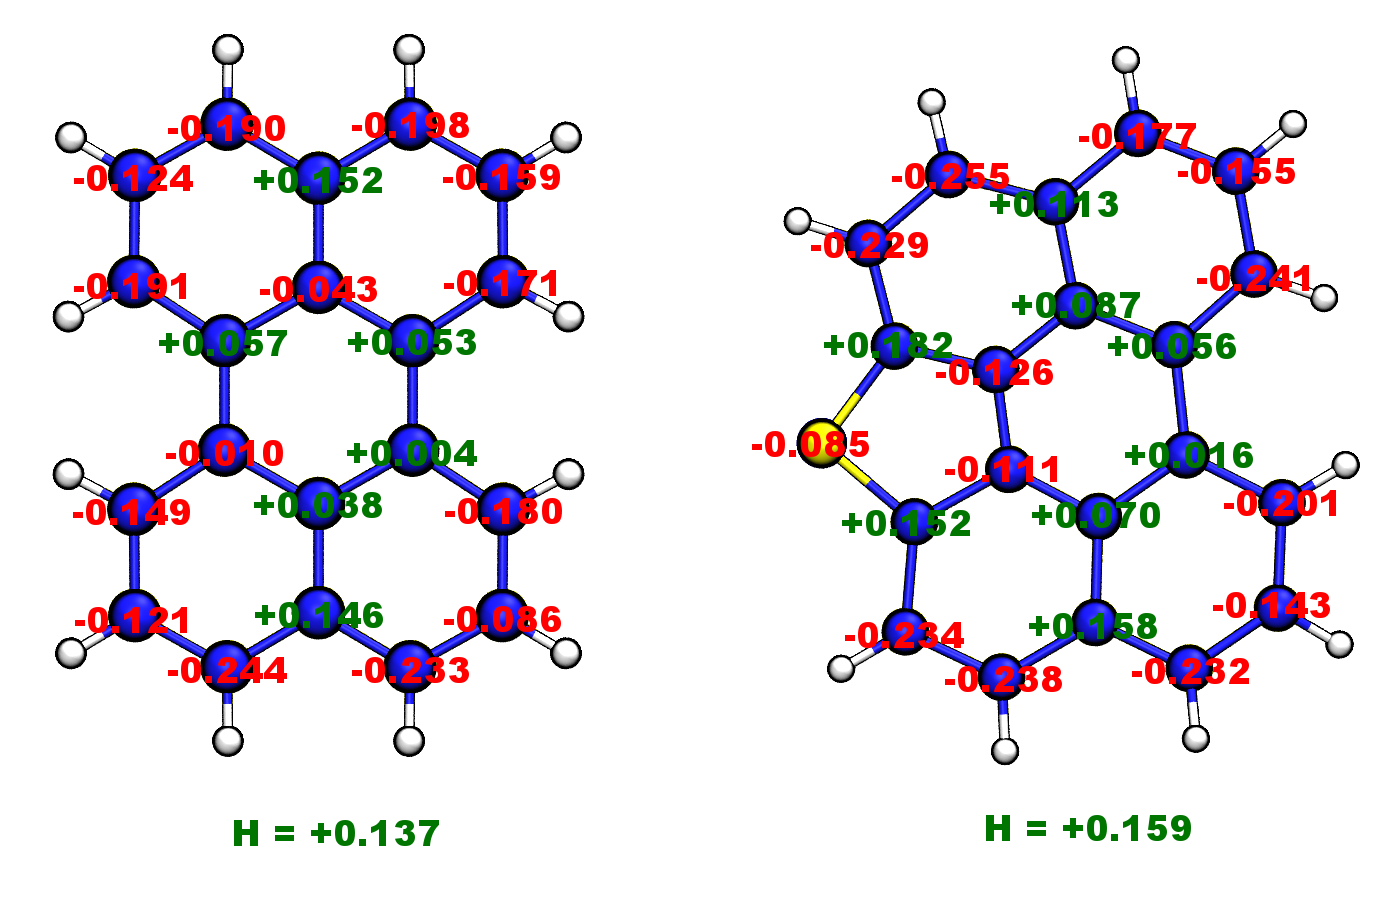
\includegraphics[width=0.85\textwidth]{Figures/chargedPAH.png}
    \caption{The charges used for the equilibration MD simulations to add charges and molecule flexibility to the previous morphologies}
	\label{fig:charges}
\end{figure}


We also explore the affect of variable-range hopping on our systems, by applying a VRH prefactor of the form $k_{ij} \propto \exp \left( - \frac{r_{ij}}{4 \text{\AA}} \right)$, which supresses hops over the long-axis of the molecules and stimulates hopping along the $\pi$-stacking direction.
The VRH decay factor (which is usuall associated with the delocalisation length) of $1 / 4 \text{\AA}$ was selected as it corresponds to the $\pi$-stacking distance, as well as the approximate chromophore size for P3HT, which we know to work well in the MorphCT pipeline.


\section{Mobility Results}


\begin{center}
\begin{adjustbox}{max width = \textwidth}
\begin{tabular}{| c | c | c | c | c | c |}
\hline
\rule{0pt}{2.5ex}
\multirow{2}{*}{\textbf{Simulation Name}}&\textbf{Density}&\textbf{Anisotropy}&\textbf{Stacks}&\textbf{Stack Threshold}&\textbf{Mobility}\\
                            &(\SI{}{\gcm})&(Arb. U.)&(Arb. U.)&(\AA)&(\SI{}{\mobunits})\\
\hhline{|======|}
{\ccg}\rule{0pt}{2.5ex}PE\_MultiStack\_Eclipsed&{\ccg}1.06&{\ccg}0.5033&{\ccg}20&{\ccg}5.06&{\ccg}7.70$\times10^{0}$\\
\rule{0pt}{2.5ex}PE\_SingleStack\_Eclipsed&1.06&0.1949&71&4.82&7.20$\times10^{-1}$\\
{\ccg}\rule{0pt}{2.5ex}PE\_SingleStack\_Ordered&{\ccg}1.06&{\ccg}0.0126&{\ccg}69&{\ccg}4.65&{\ccg}1.64$\times10^{-1}$\\
\hhline{------}
\rule{0pt}{2.5ex}PT\_MultiStack\_Eclipsed&1.01&0.0954&21&5.31&5.54$\times10^{0}$\\
{\ccg}\rule{0pt}{2.5ex}PT\_MultiStack\_Ordered&{\ccg}1.01&{\ccg}0.0058&{\ccg}75&{\ccg}4.83&{\ccg}7.58$\times10^{0}$\\
\rule{0pt}{2.5ex}PT\_SingleStack\_Eclipsed&1.01&0.1018&2&5.14&5.16$\times10^{0}$\\
{\ccg}\rule{0pt}{2.5ex}PT\_SingleStack\_Ordered&{\ccg}1.01&{\ccg}0.0547&{\ccg}6&{\ccg}5.18&{\ccg}5.47$\times10^{0}$\\
\hhline{|======|}
\rule{0pt}{2.5ex}VRH\_PE\_MultiStack\_Eclipsed&1.06&0.3877&20&5.06&5.33$\times10^{-1}$\\
{\ccg}\rule{0pt}{2.5ex}VRH\_PE\_SingleStack\_Eclipsed&{\ccg}1.06&{\ccg}0.0935&{\ccg}71&{\ccg}4.82&{\ccg}6.21$\times10^{-2}$\\
\rule{0pt}{2.5ex}VRH\_PE\_SingleStack\_Ordered&1.06&0.0027&69&4.65&1.33$\times10^{-2}$\\
\hhline{------}
{\ccg}\rule{0pt}{2.5ex}VRH\_PT\_MultiStack\_Eclipsed&{\ccg}1.01&{\ccg}0.0861&{\ccg}21&{\ccg}5.31&{\ccg}5.72$\times10^{-1}$\\
\rule{0pt}{2.5ex}VRH\_PT\_MultiStack\_Ordered&1.01&0.0039&75&4.83&8.35$\times10^{-1}$\\
{\ccg}\rule{0pt}{2.5ex}VRH\_PT\_SingleStack\_Eclipsed&{\ccg}1.01&{\ccg}0.0344&{\ccg}2&{\ccg}5.14&{\ccg}4.84$\times10^{-1}$\\
\rule{0pt}{2.5ex}VRH\_PT\_SingleStack\_Ordered&1.01&0.1455&6&5.18&5.47$\times10^{-1}$\\
\hhline{------}
\end{tabular}\label{table:mob}
\end{adjustbox}
\captionof{table}{The results from MorphCT for the various flexible, charged PAH morphologies with variable ranged hopping (VRH) corrections on or off.}
\end{center}

\clearpage

\section{Analysis Figures with VRH off}

\begin{figure}[h]\centering
	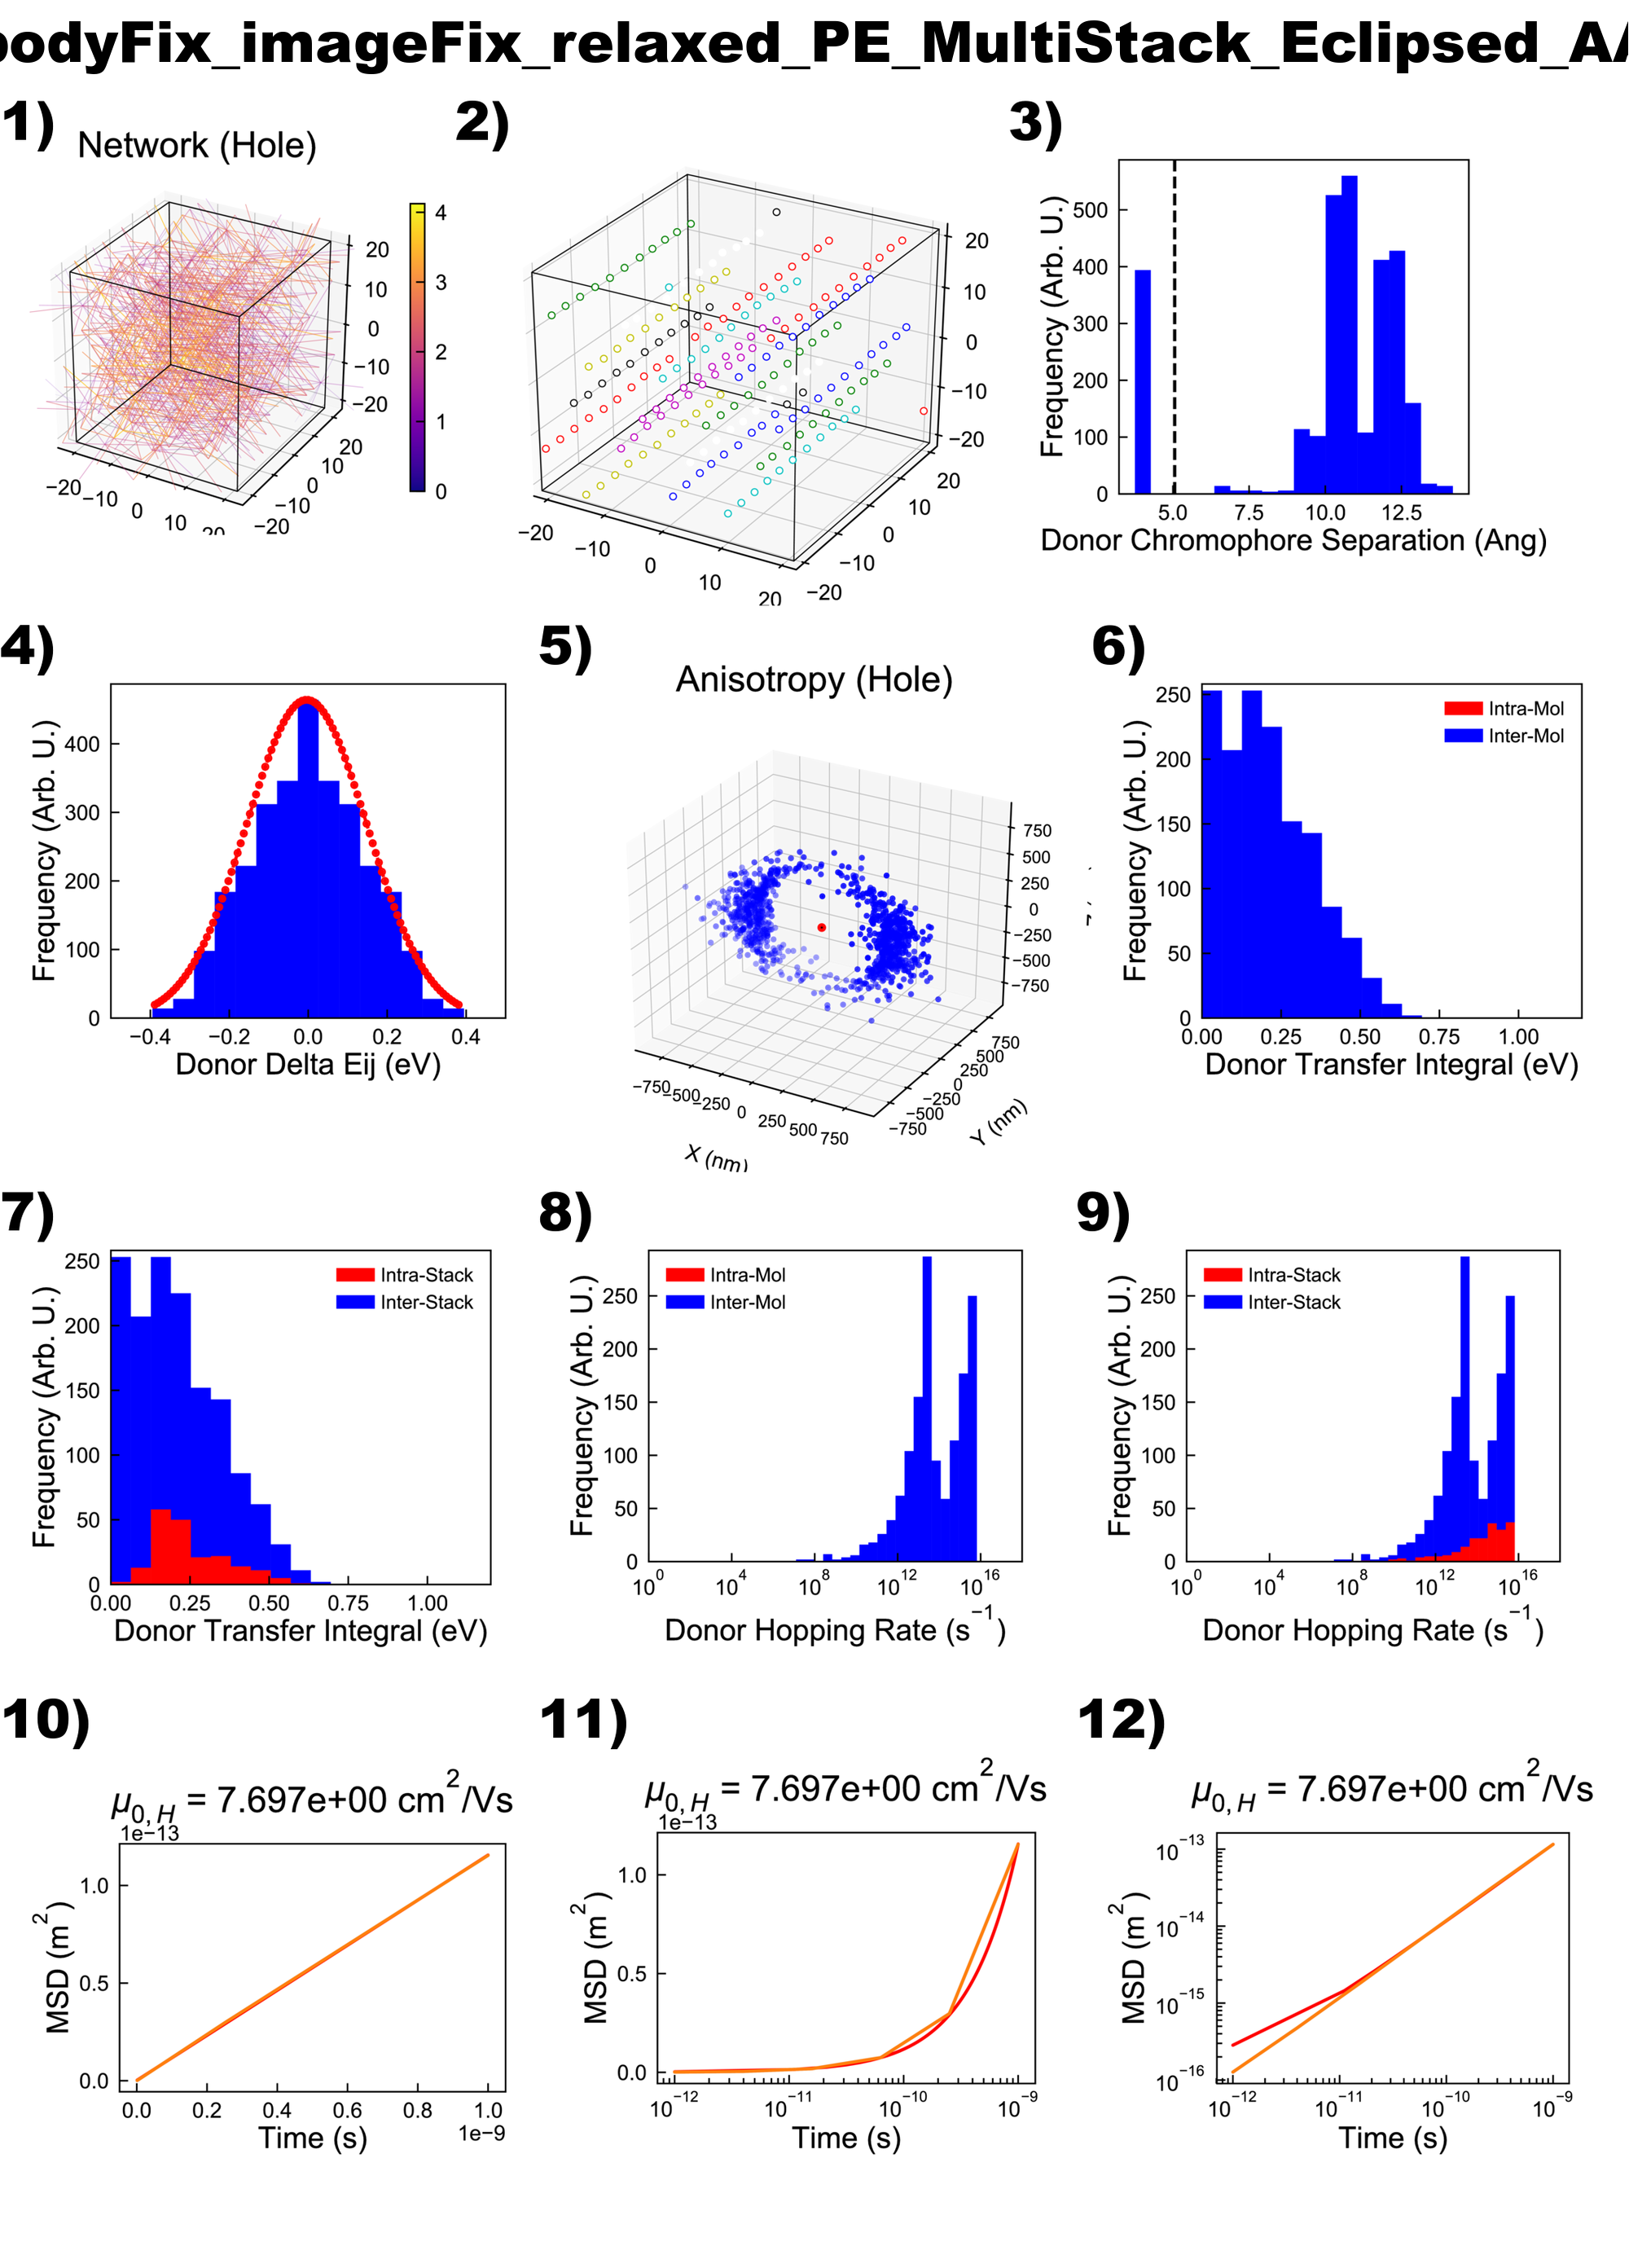
\includegraphics[width=0.65\textwidth]{Figures/bodyFix_imageFix_relaxed_PE_MultiStack_Eclipsed_AA.png}
    \caption{   1) Chromophore connectivity network, 
                2) Location of `stacks', 
                3) Distribution of connected chromophore separations (defines stacks),
                4) Density of states of Frontier molecular orbital (delta Eij),
                5) KMC Carrier termination locations (defines anisotropy),
                6) Histogram of molecular transfer integrals,
                7) Histogram of stack transfer integrals,
                8) Histogram of molecular hopping rates,
                9) Histogram of stack hopping rates,
                10) Linear MSD plot,
                11) Semi-log-x MSD plot,
                12) Logarithmic MSD plot.}
	\label{fig:PEMultEcl}
\end{figure}


\begin{figure}[h]\centering
	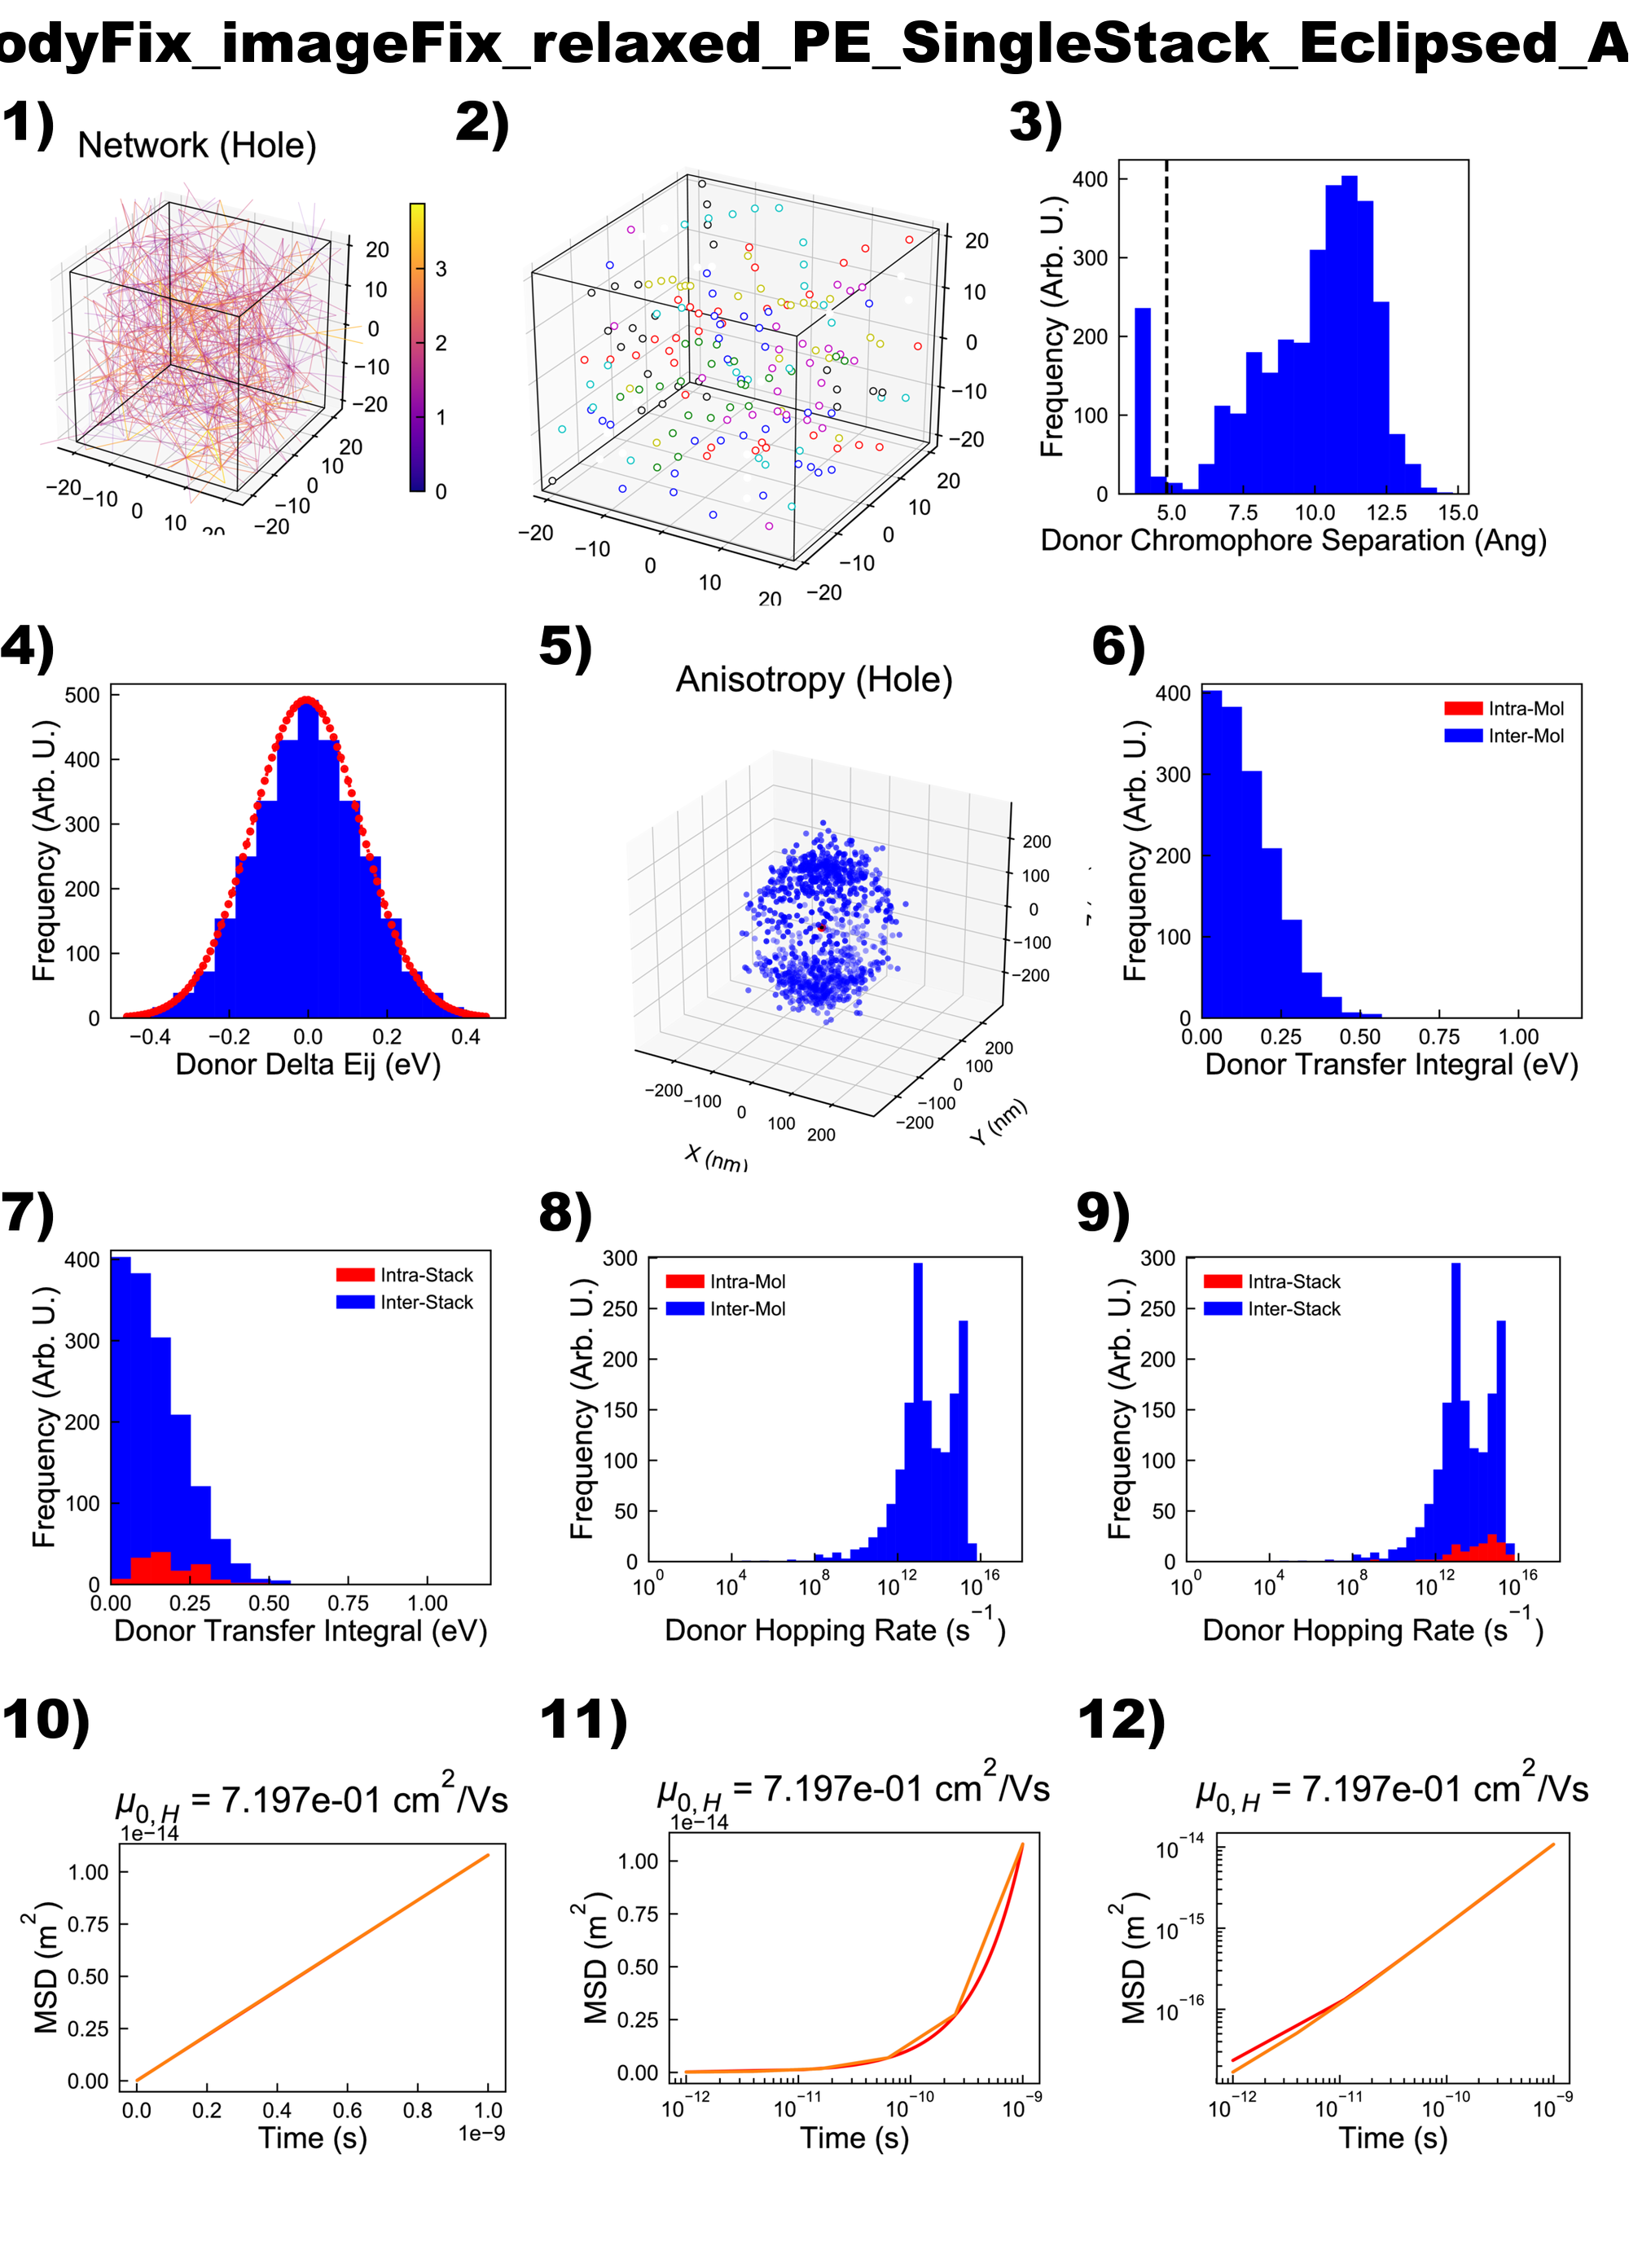
\includegraphics[width=0.85\textwidth]{Figures/bodyFix_imageFix_relaxed_PE_SingleStack_Eclipsed_AA.png}
    \caption{   1) Chromophore connectivity network, 
                2) Location of `stacks', 
                3) Distribution of connected chromophore separations (defines stacks),
                4) Density of states of Frontier molecular orbital (delta Eij),
                5) KMC Carrier termination locations (defines anisotropy),
                6) Histogram of molecular transfer integrals,
                7) Histogram of stack transfer integrals,
                8) Histogram of molecular hopping rates,
                9) Histogram of stack hopping rates,
                10) Linear MSD plot,
                11) Semi-log-x MSD plot,
                12) Logarithmic MSD plot.}
	\label{fig:PESingEcl}
\end{figure}


\begin{figure}[h]\centering
	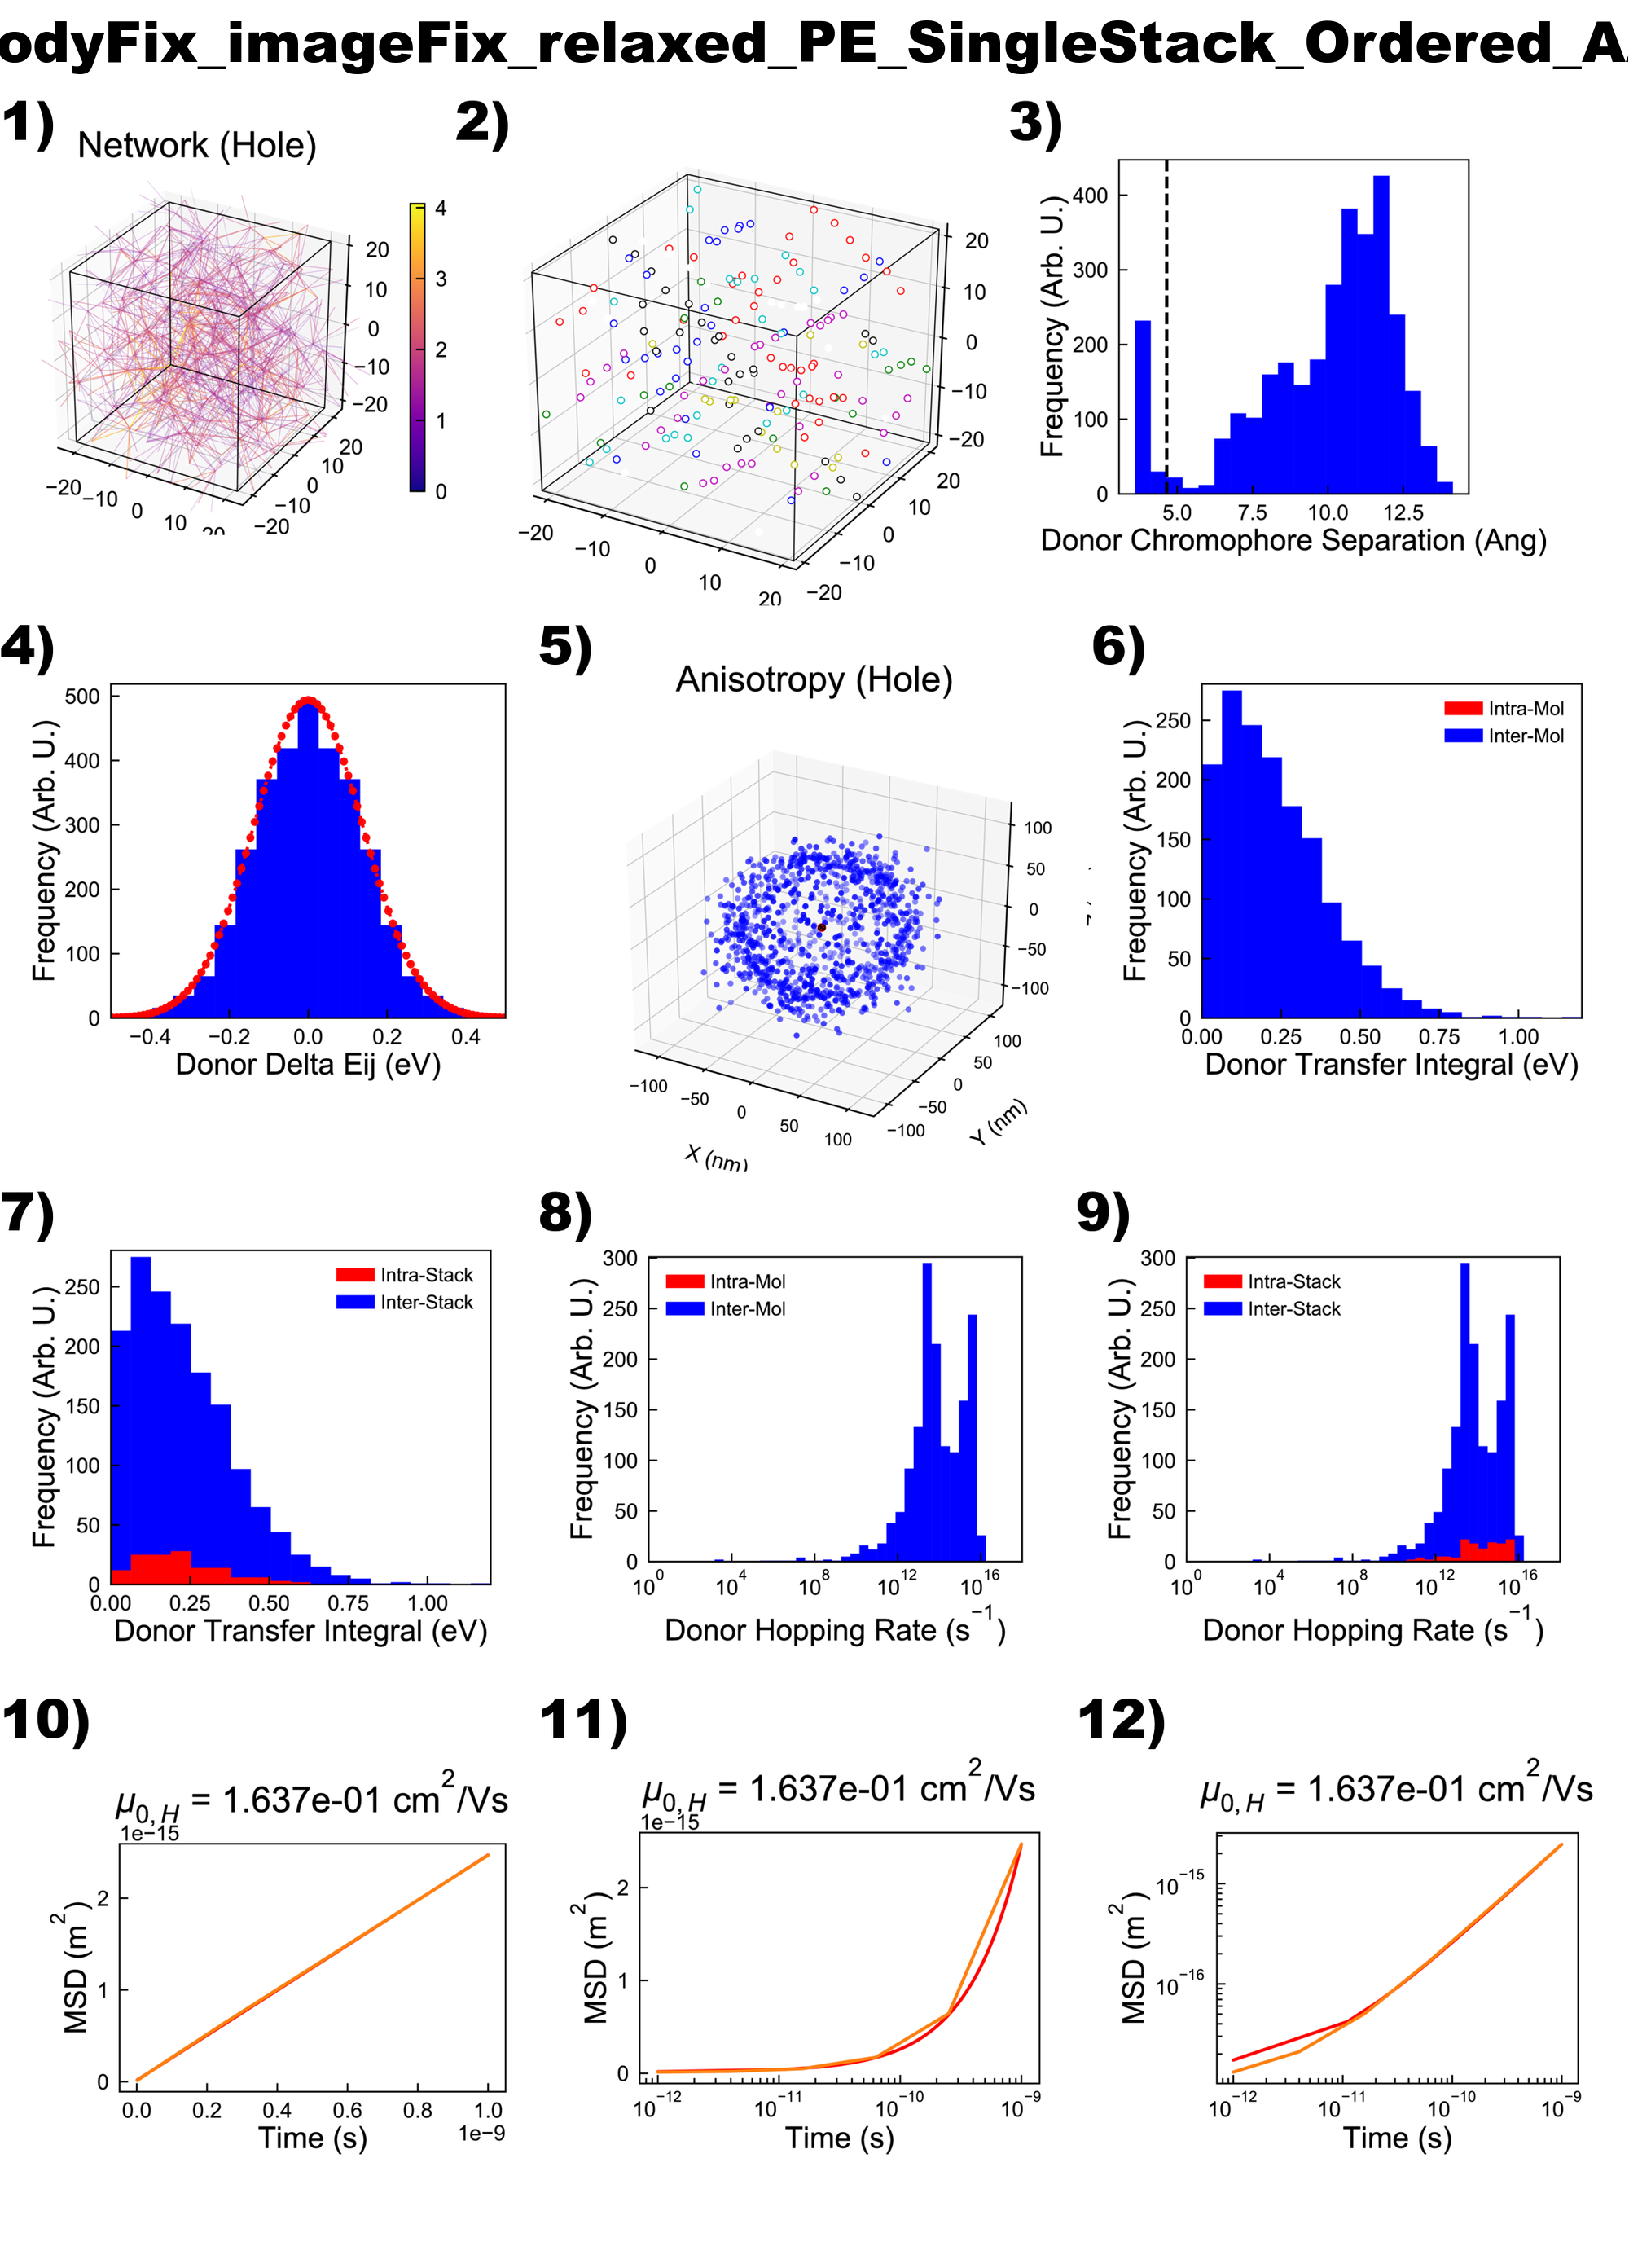
\includegraphics[width=0.85\textwidth]{Figures/bodyFix_imageFix_relaxed_PE_SingleStack_Ordered_AA.png}
    \caption{   1) Chromophore connectivity network, 
                2) Location of `stacks', 
                3) Distribution of connected chromophore separations (defines stacks),
                4) Density of states of Frontier molecular orbital (delta Eij),
                5) KMC Carrier termination locations (defines anisotropy),
                6) Histogram of molecular transfer integrals,
                7) Histogram of stack transfer integrals,
                8) Histogram of molecular hopping rates,
                9) Histogram of stack hopping rates,
                10) Linear MSD plot,
                11) Semi-log-x MSD plot,
                12) Logarithmic MSD plot.}
	\label{fig:PESingOrd}
\end{figure}


\begin{figure}[h]\centering
	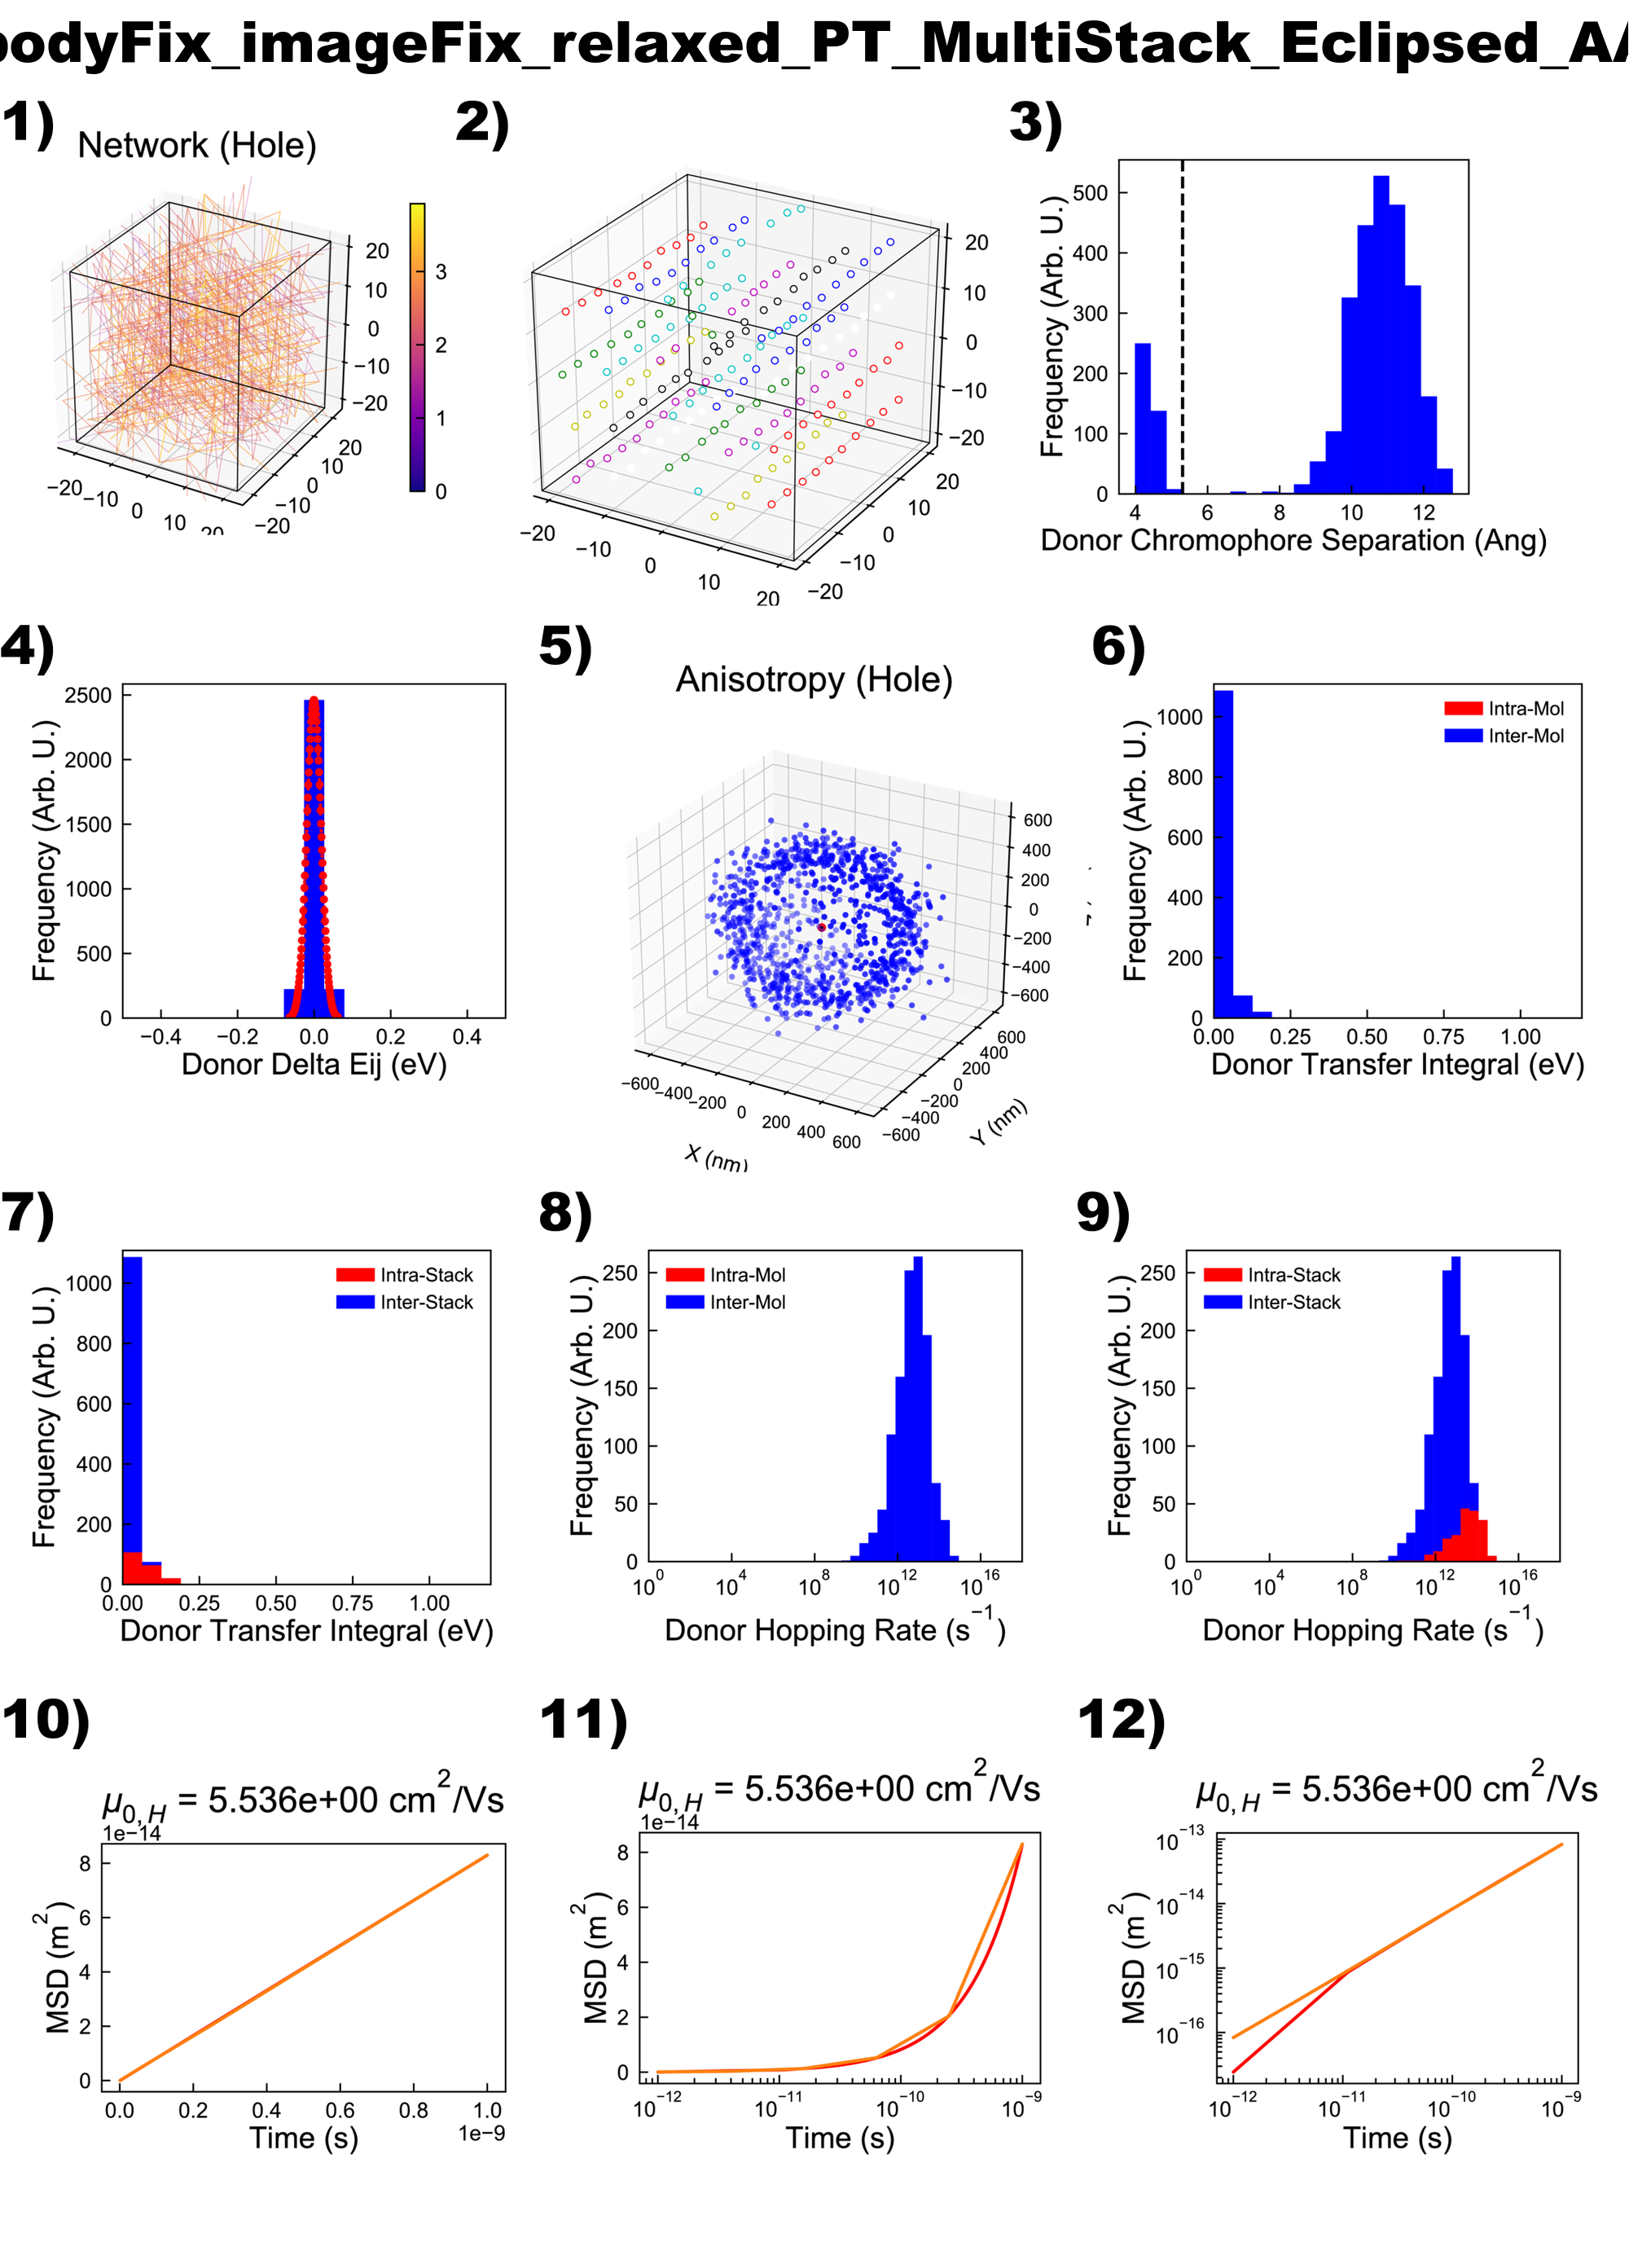
\includegraphics[width=0.85\textwidth]{Figures/bodyFix_imageFix_relaxed_PT_MultiStack_Eclipsed_AA.png}
    \caption{   1) Chromophore connectivity network, 
                2) Location of `stacks', 
                3) Distribution of connected chromophore separations (defines stacks),
                4) Density of states of Frontier molecular orbital (delta Eij),
                5) KMC Carrier termination locations (defines anisotropy),
                6) Histogram of molecular transfer integrals,
                7) Histogram of stack transfer integrals,
                8) Histogram of molecular hopping rates,
                9) Histogram of stack hopping rates,
                10) Linear MSD plot,
                11) Semi-log-x MSD plot,
                12) Logarithmic MSD plot.}
	\label{fig:PTMultEcl}
\end{figure}


\begin{figure}[h]\centering
	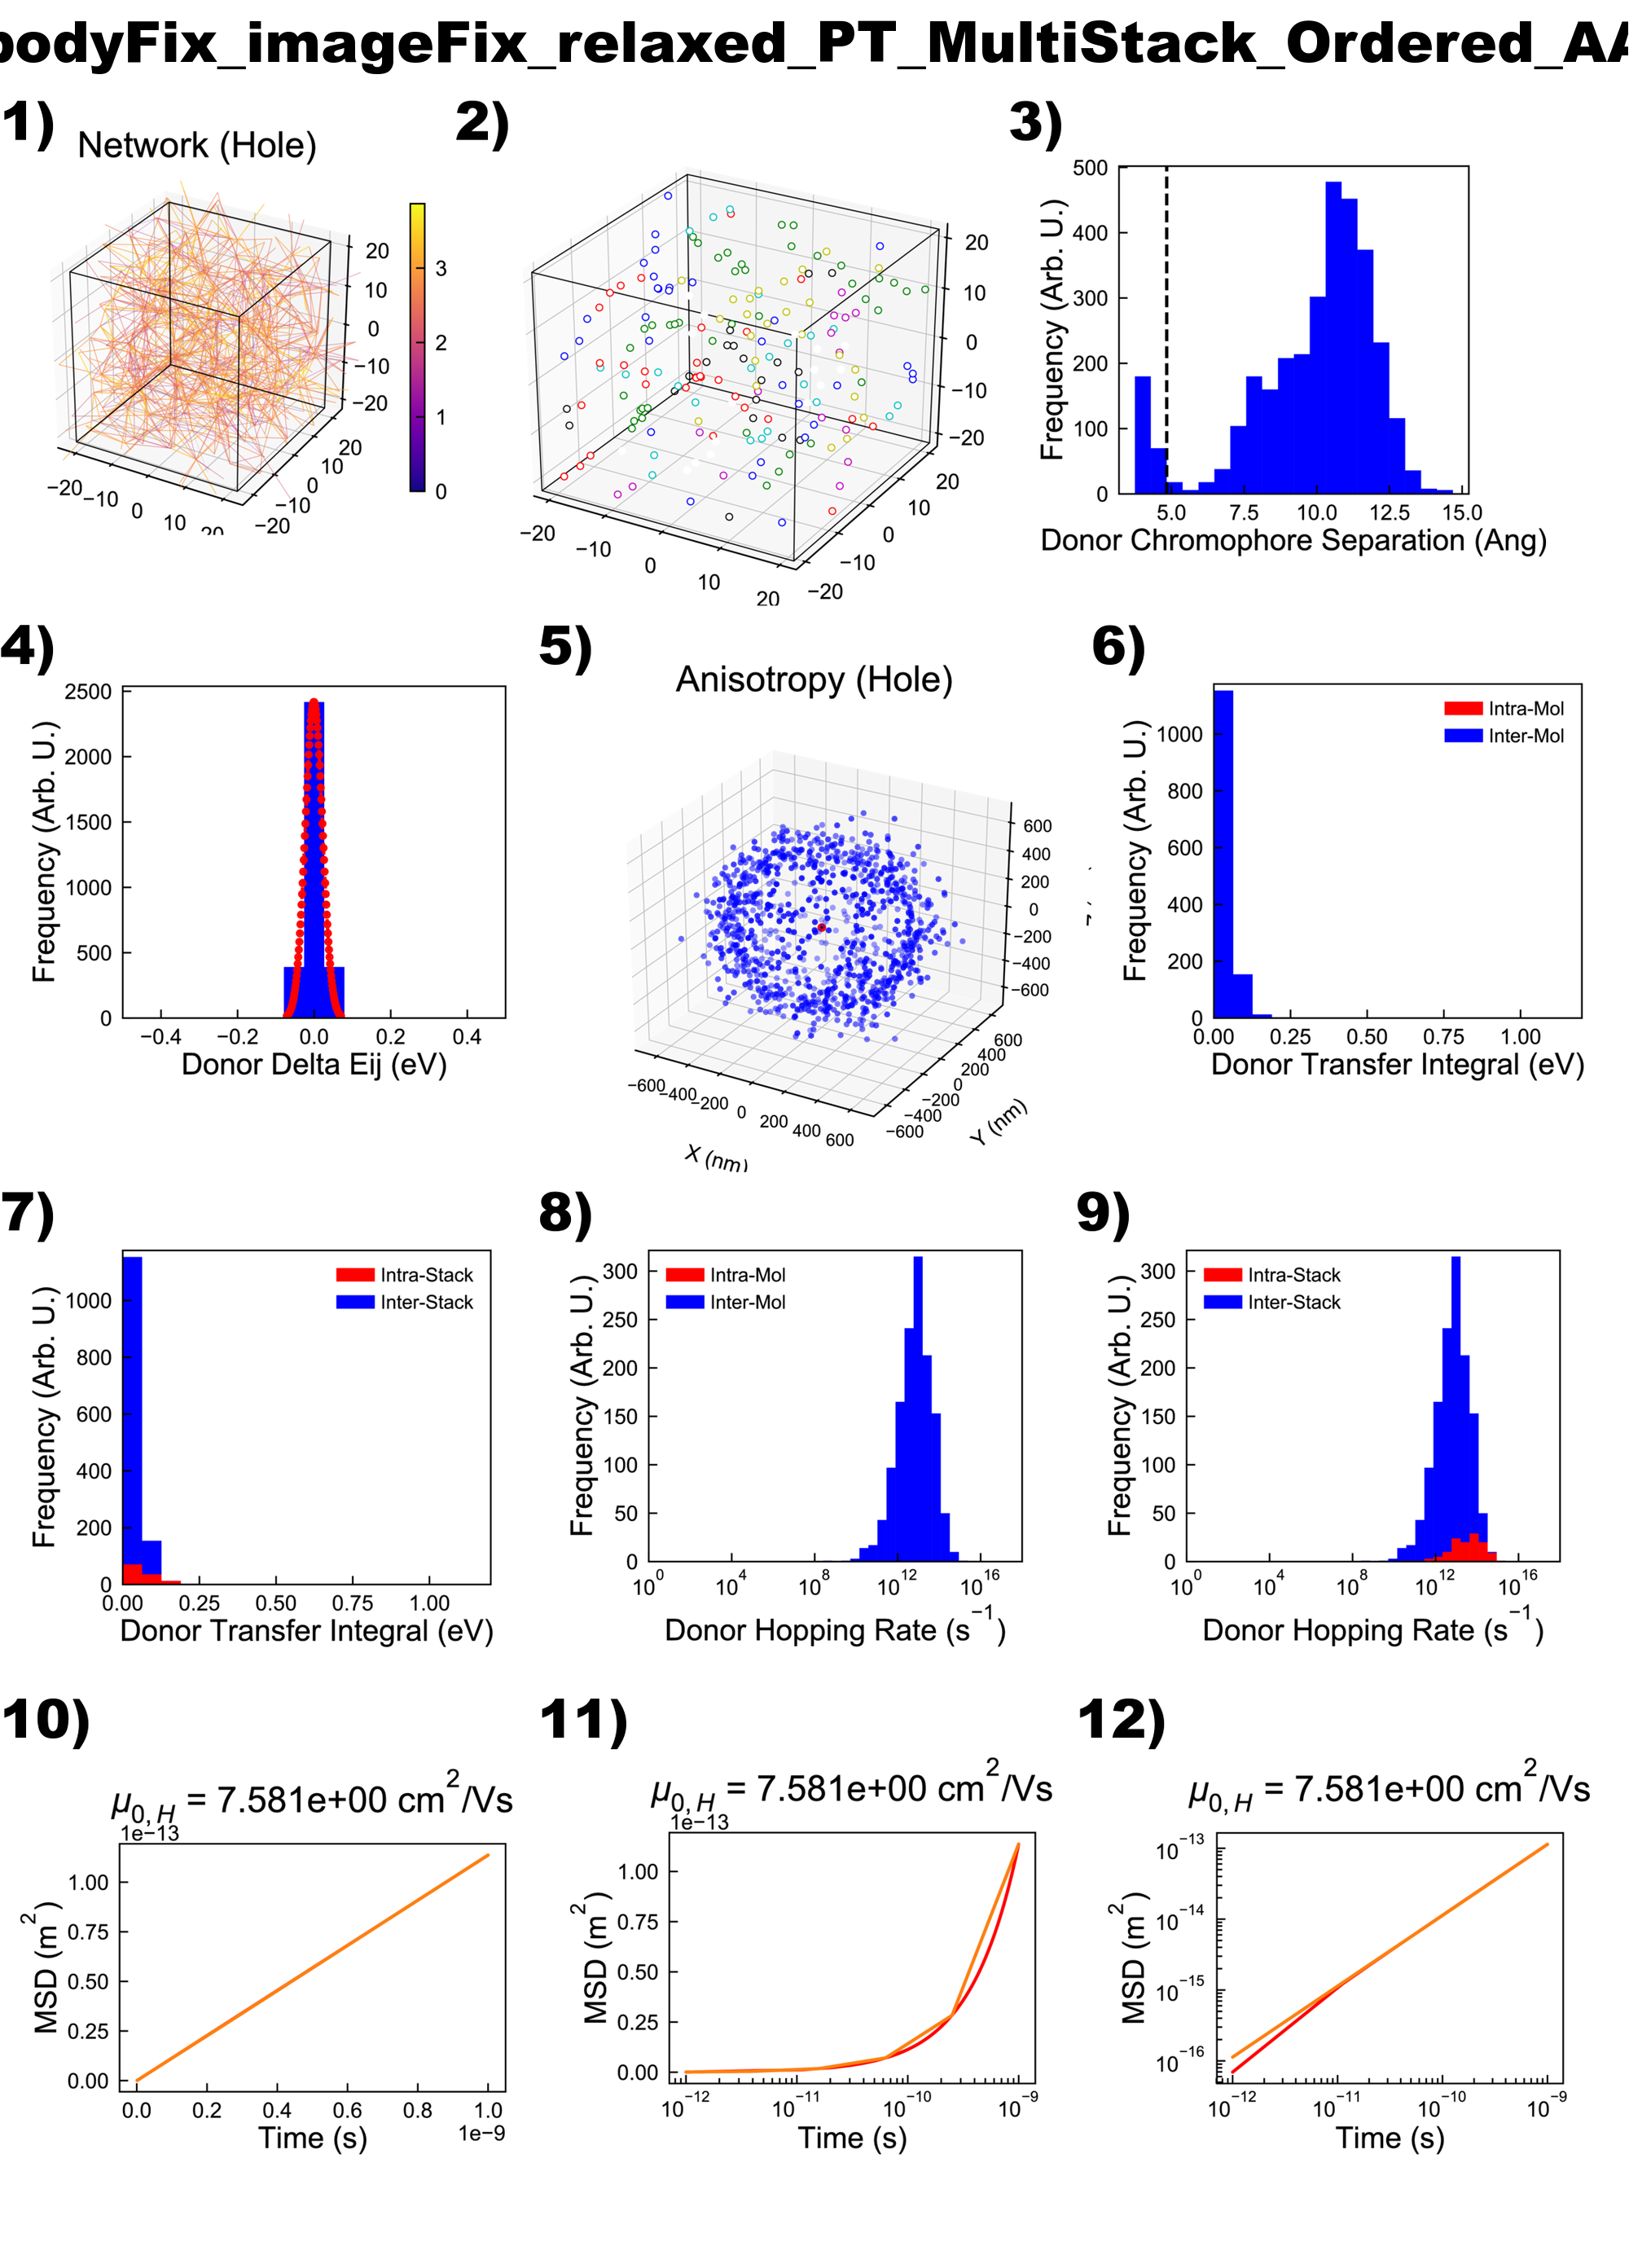
\includegraphics[width=0.85\textwidth]{Figures/bodyFix_imageFix_relaxed_PT_MultiStack_Ordered_AA.png}
    \caption{   1) Chromophore connectivity network, 
                2) Location of `stacks', 
                3) Distribution of connected chromophore separations (defines stacks),
                4) Density of states of Frontier molecular orbital (delta Eij),
                5) KMC Carrier termination locations (defines anisotropy),
                6) Histogram of molecular transfer integrals,
                7) Histogram of stack transfer integrals,
                8) Histogram of molecular hopping rates,
                9) Histogram of stack hopping rates,
                10) Linear MSD plot,
                11) Semi-log-x MSD plot,
                12) Logarithmic MSD plot.}
	\label{fig:PTMultOrd}
\end{figure}


\begin{figure}[h]\centering
	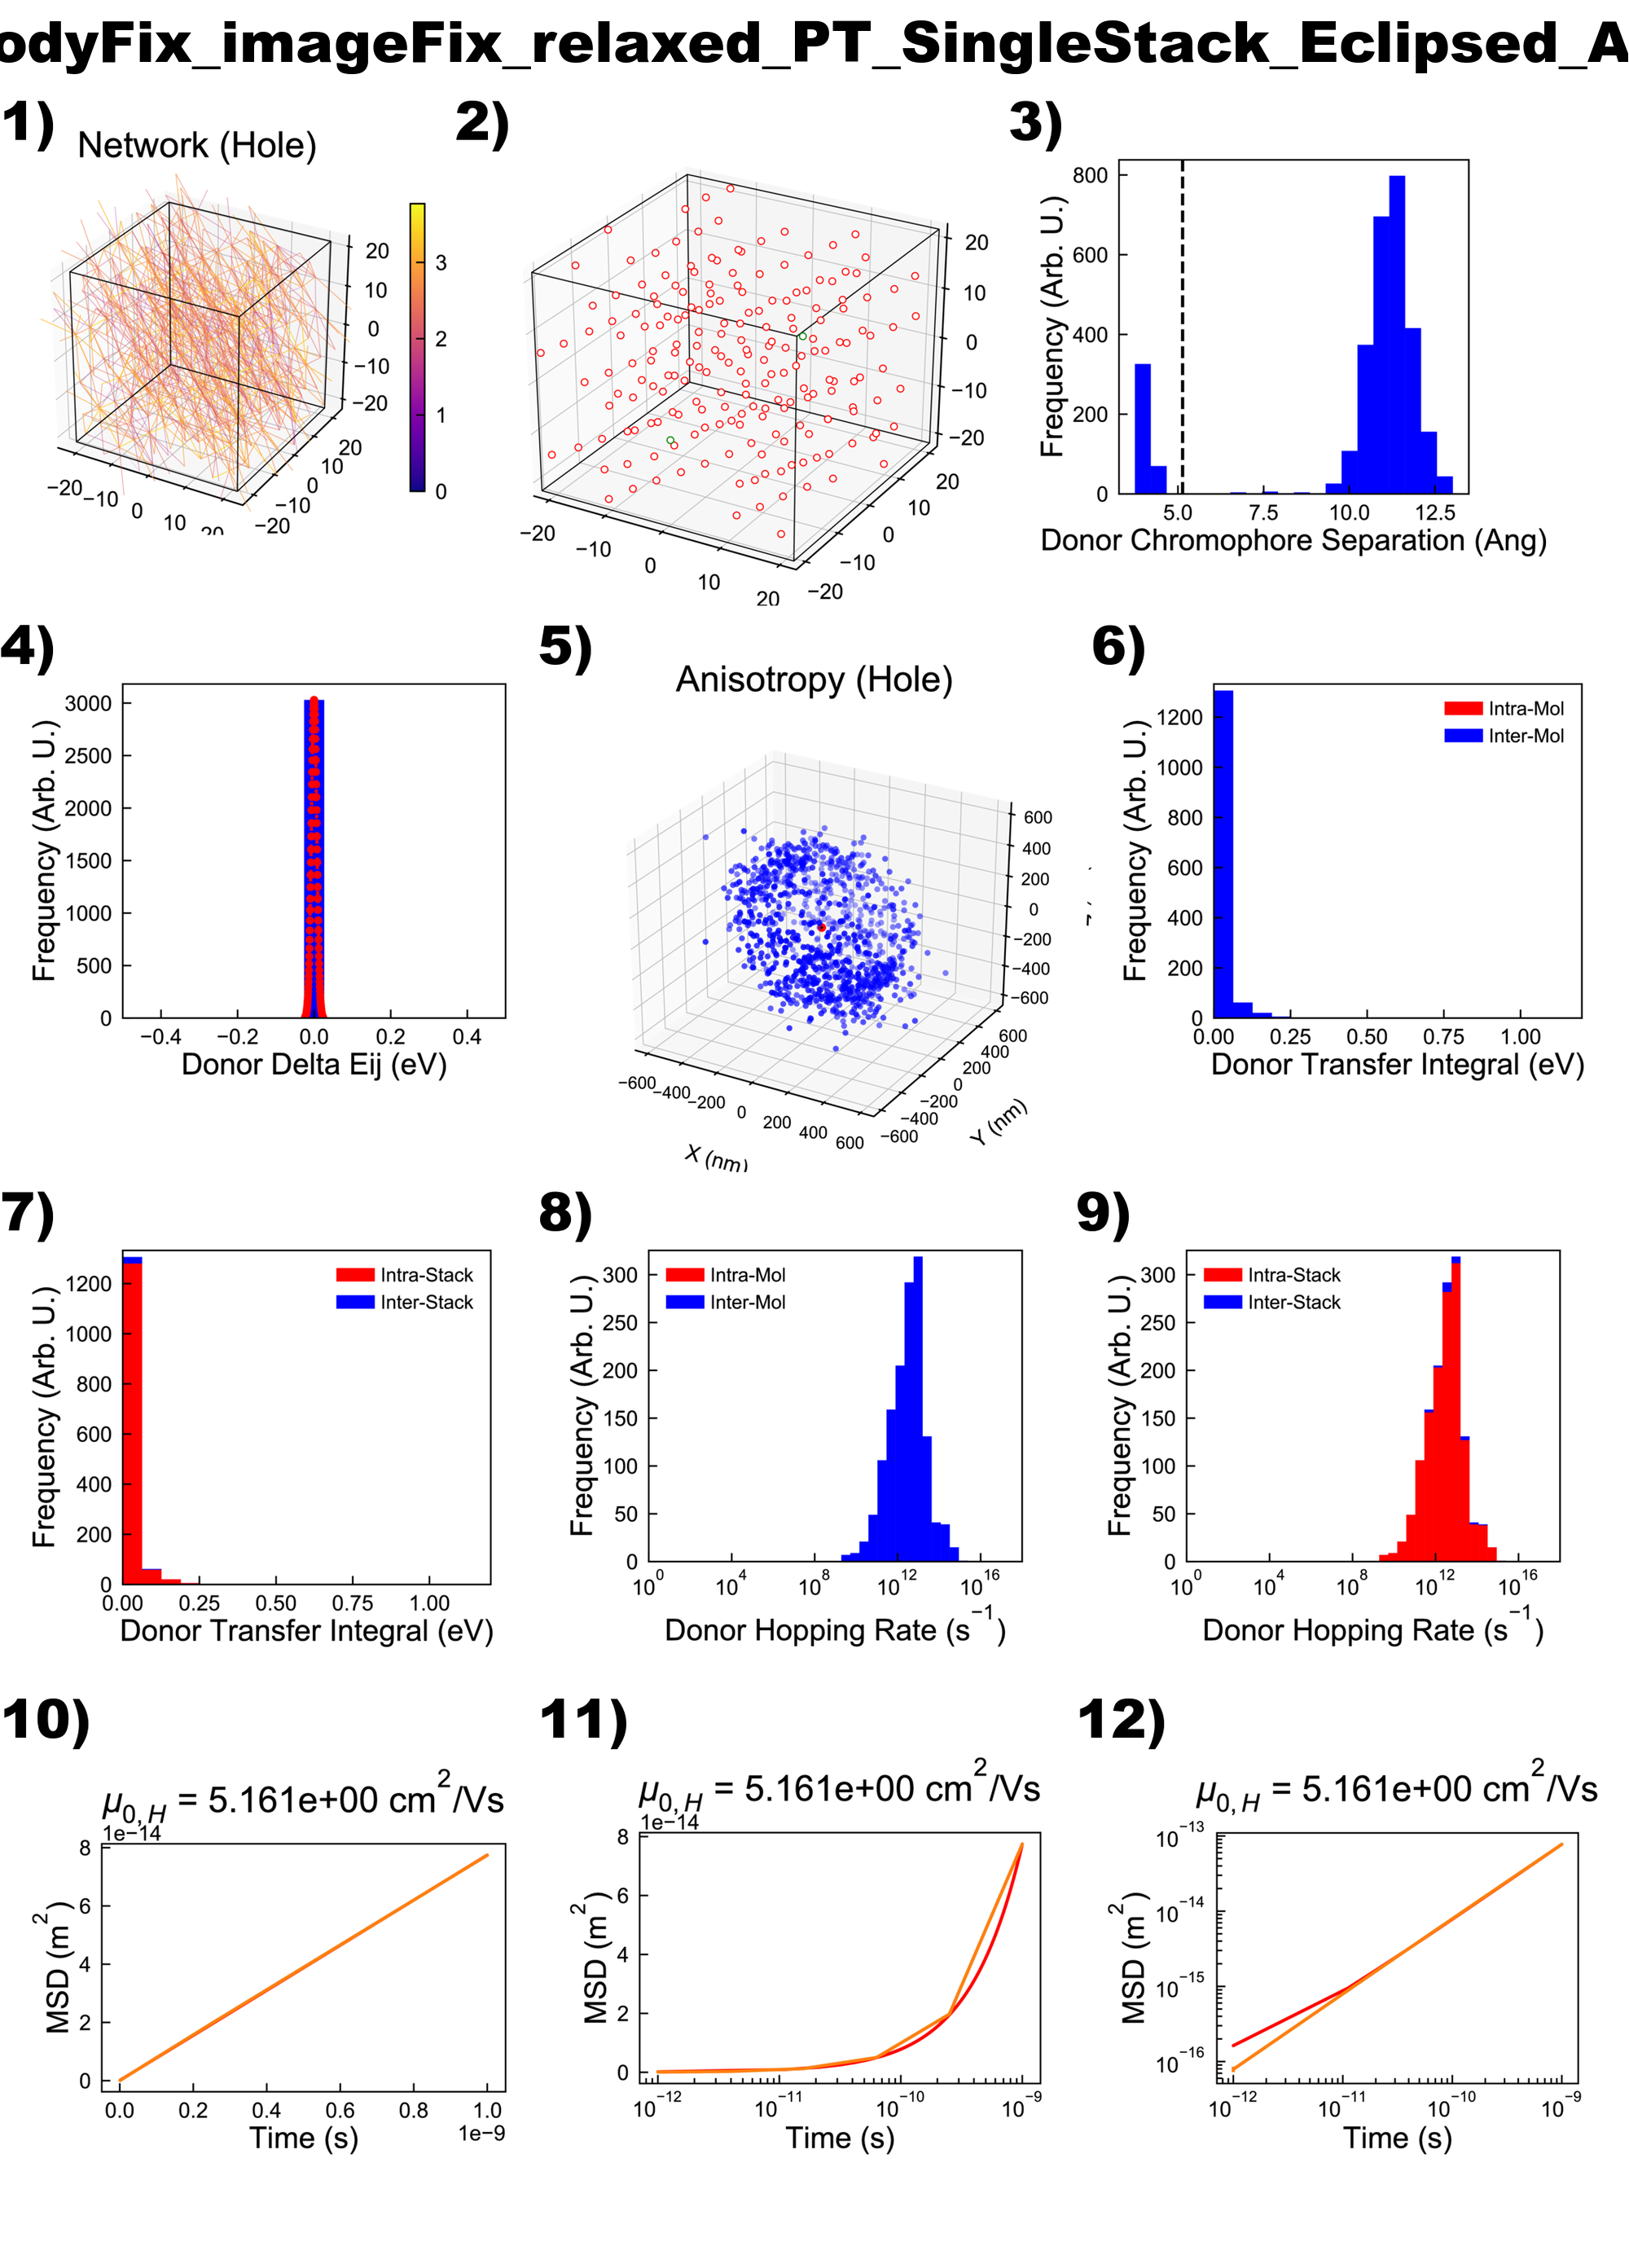
\includegraphics[width=0.85\textwidth]{Figures/bodyFix_imageFix_relaxed_PT_SingleStack_Eclipsed_AA.png}
    \caption{   1) Chromophore connectivity network, 
                2) Location of `stacks', 
                3) Distribution of connected chromophore separations (defines stacks),
                4) Density of states of Frontier molecular orbital (delta Eij),
                5) KMC Carrier termination locations (defines anisotropy),
                6) Histogram of molecular transfer integrals,
                7) Histogram of stack transfer integrals,
                8) Histogram of molecular hopping rates,
                9) Histogram of stack hopping rates,
                10) Linear MSD plot,
                11) Semi-log-x MSD plot,
                12) Logarithmic MSD plot.}
	\label{fig:PTSingEcl}
\end{figure}


\begin{figure}[h]\centering
	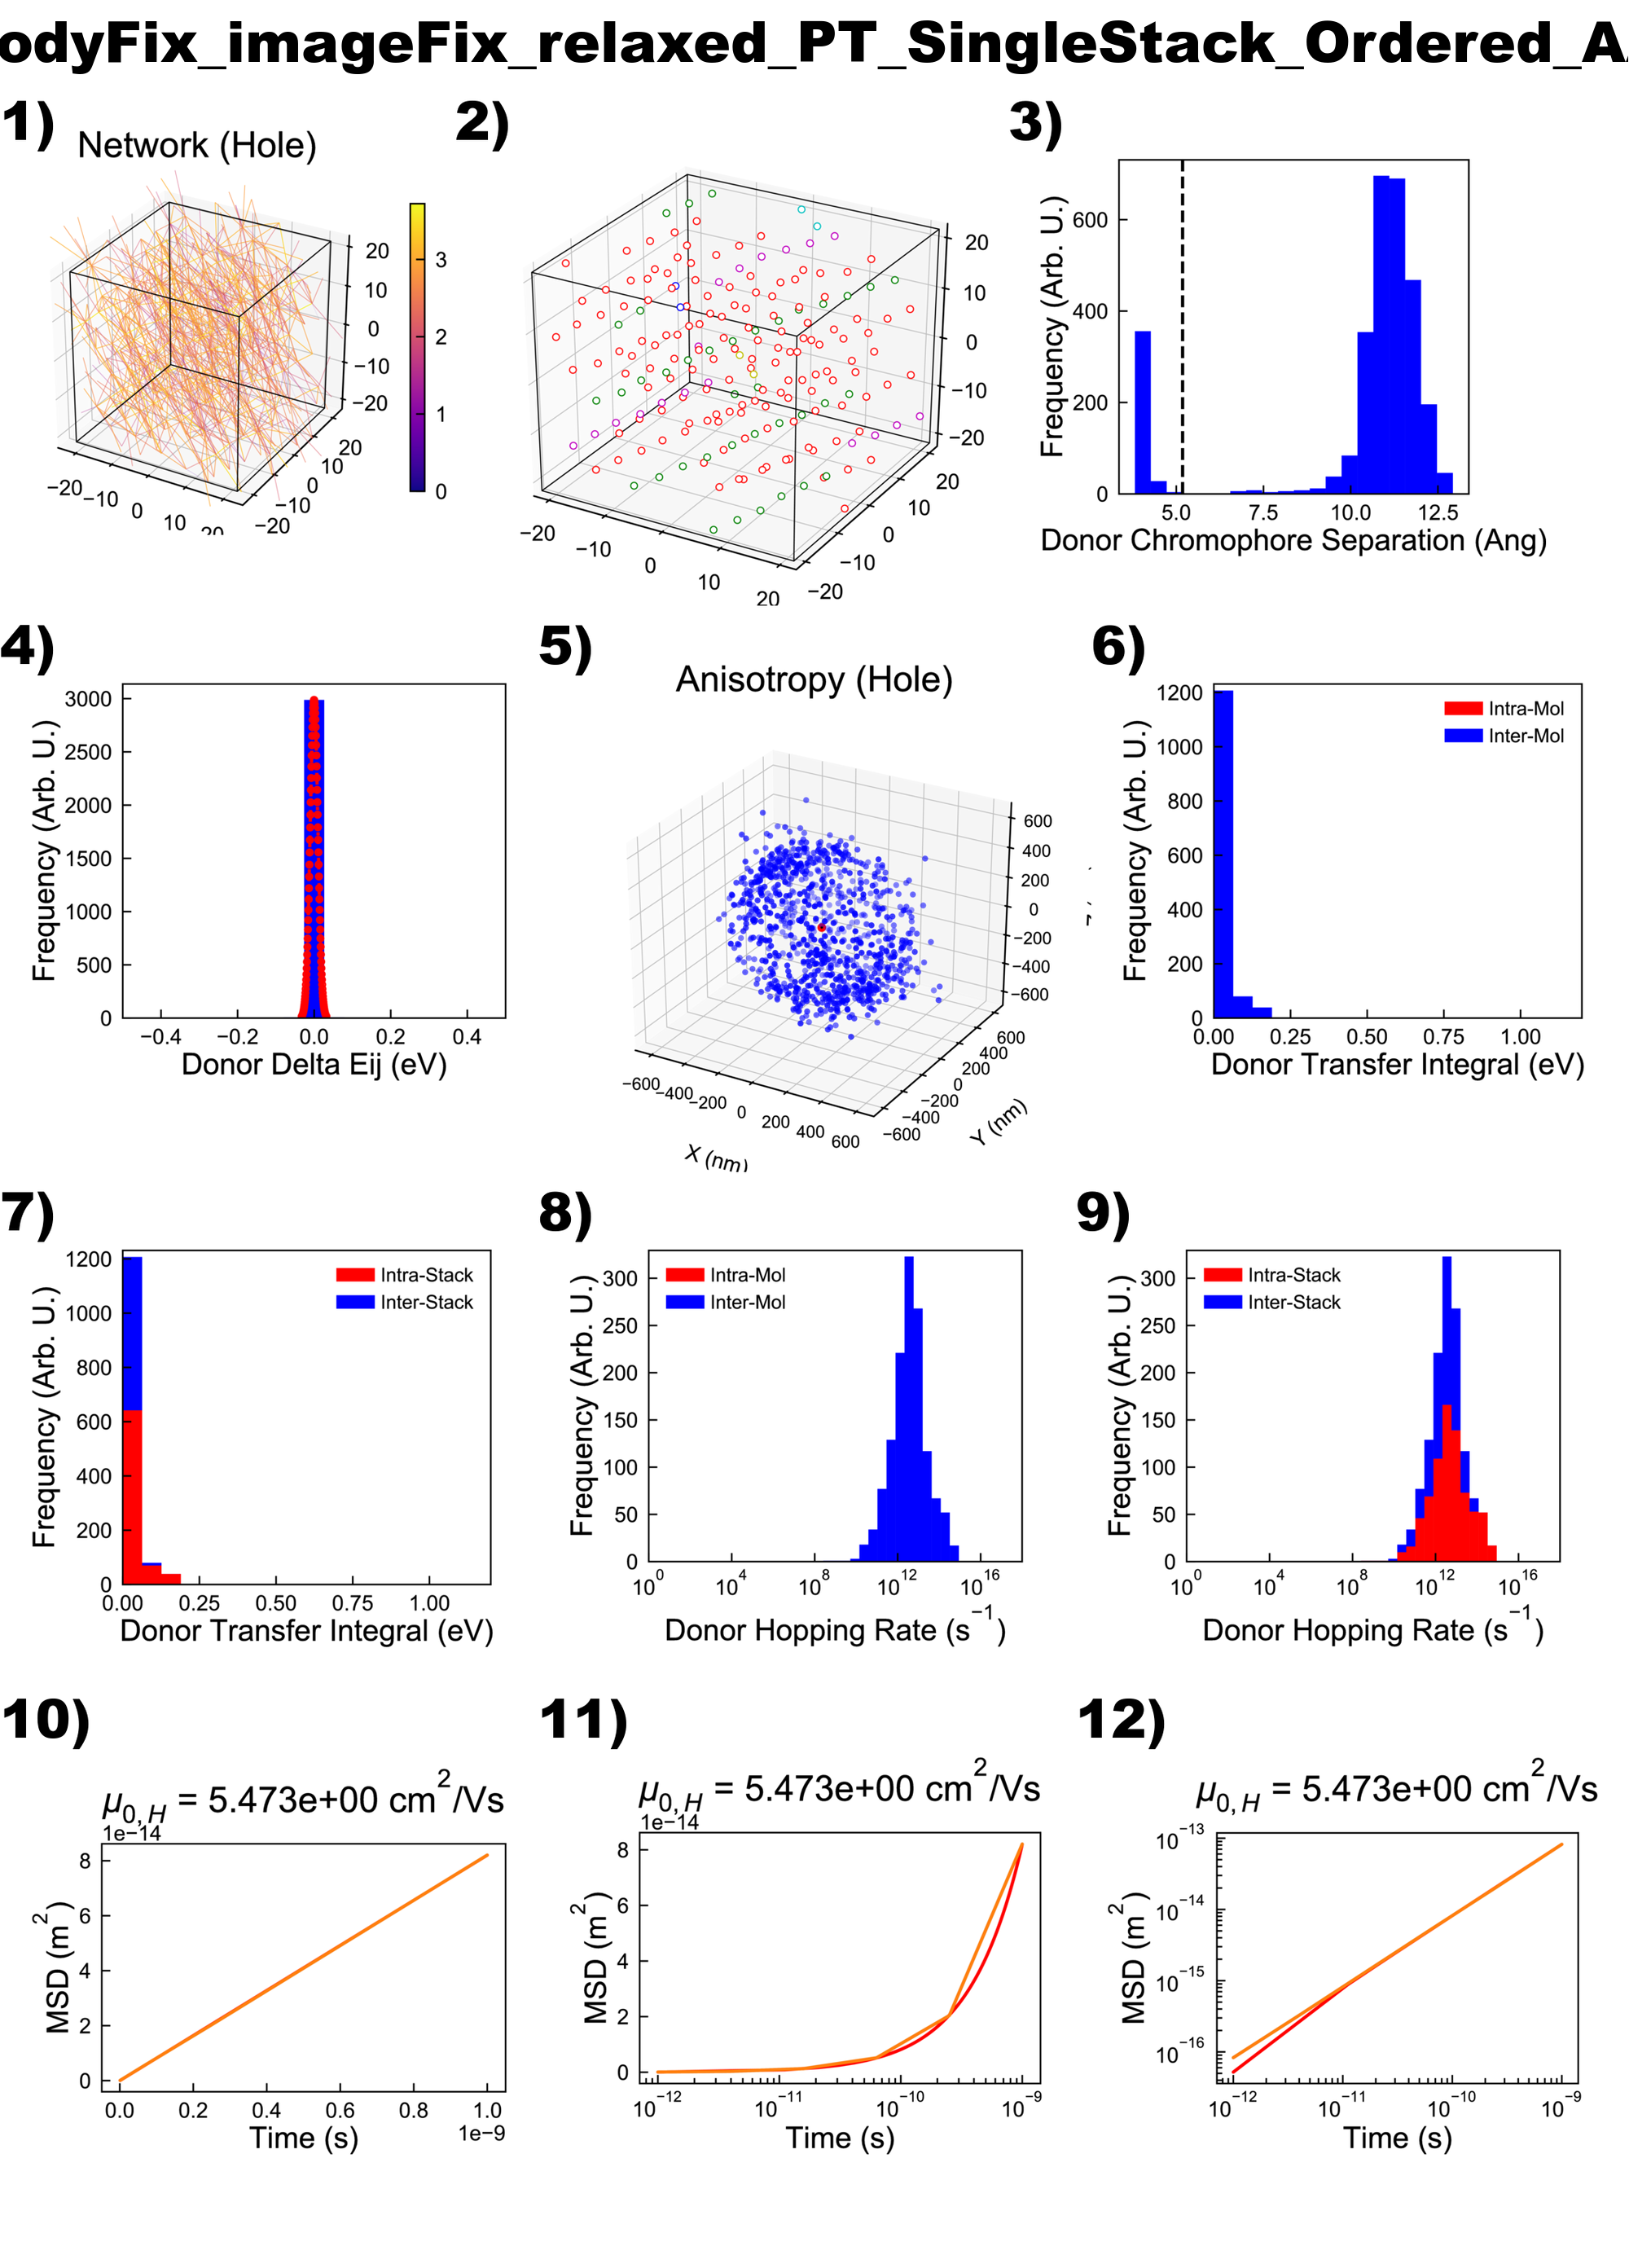
\includegraphics[width=0.85\textwidth]{Figures/bodyFix_imageFix_relaxed_PT_SingleStack_Ordered_AA.png}
    \caption{   1) Chromophore connectivity network, 
                2) Location of `stacks', 
                3) Distribution of connected chromophore separations (defines stacks),
                4) Density of states of Frontier molecular orbital (delta Eij),
                5) KMC Carrier termination locations (defines anisotropy),
                6) Histogram of molecular transfer integrals,
                7) Histogram of stack transfer integrals,
                8) Histogram of molecular hopping rates,
                9) Histogram of stack hopping rates,
                10) Linear MSD plot,
                11) Semi-log-x MSD plot,
                12) Logarithmic MSD plot.}
	\label{fig:PTSingOrd}
\end{figure}

\clearpage
\section{Analysis Figures with VRH on}

\begin{figure}[h]\centering
	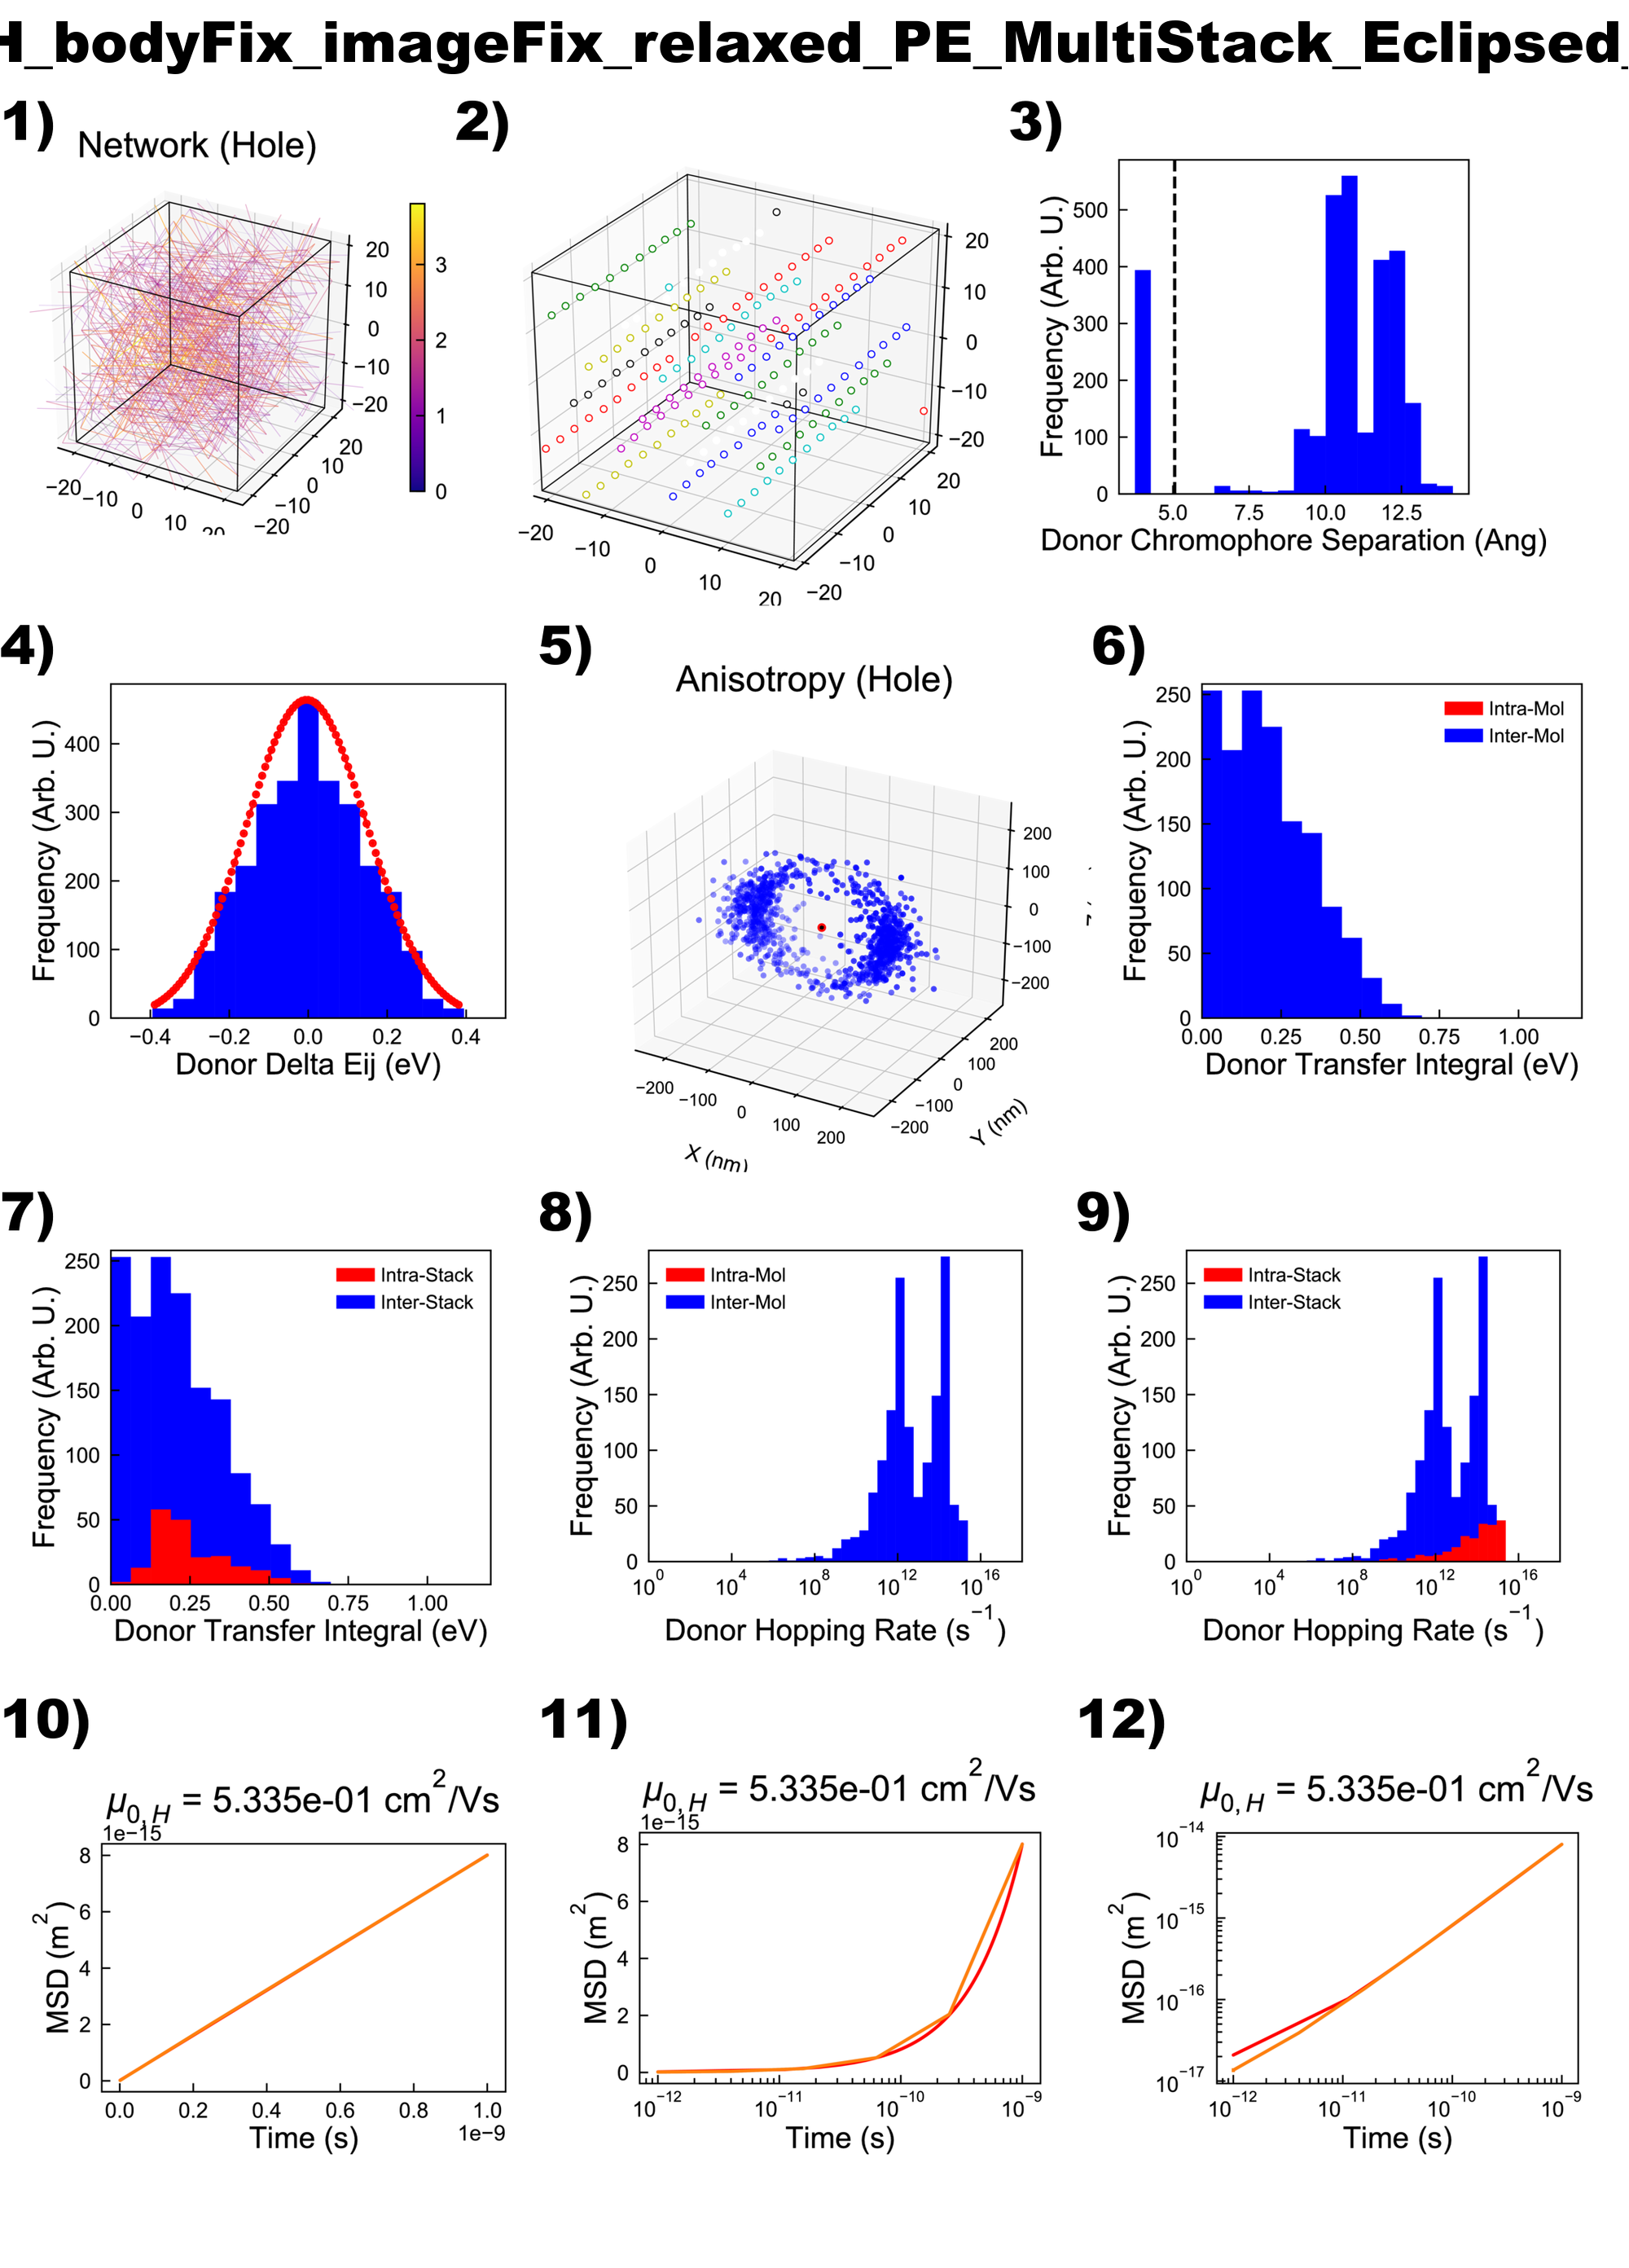
\includegraphics[width=0.65\textwidth]{Figures/VRH_bodyFix_imageFix_relaxed_PE_MultiStack_Eclipsed_AA.png}
    \caption{   1) Chromophore connectivity network, 
                2) Location of `stacks', 
                3) Distribution of connected chromophore separations (defines stacks),
                4) Density of states of Frontier molecular orbital (delta Eij),
                5) KMC Carrier termination locations (defines anisotropy),
                6) Histogram of molecular transfer integrals,
                7) Histogram of stack transfer integrals,
                8) Histogram of molecular hopping rates,
                9) Histogram of stack hopping rates,
                10) Linear MSD plot,
                11) Semi-log-x MSD plot,
                12) Logarithmic MSD plot.}
	\label{fig:VRHPEMultEcl}
\end{figure}


\begin{figure}[h]\centering
	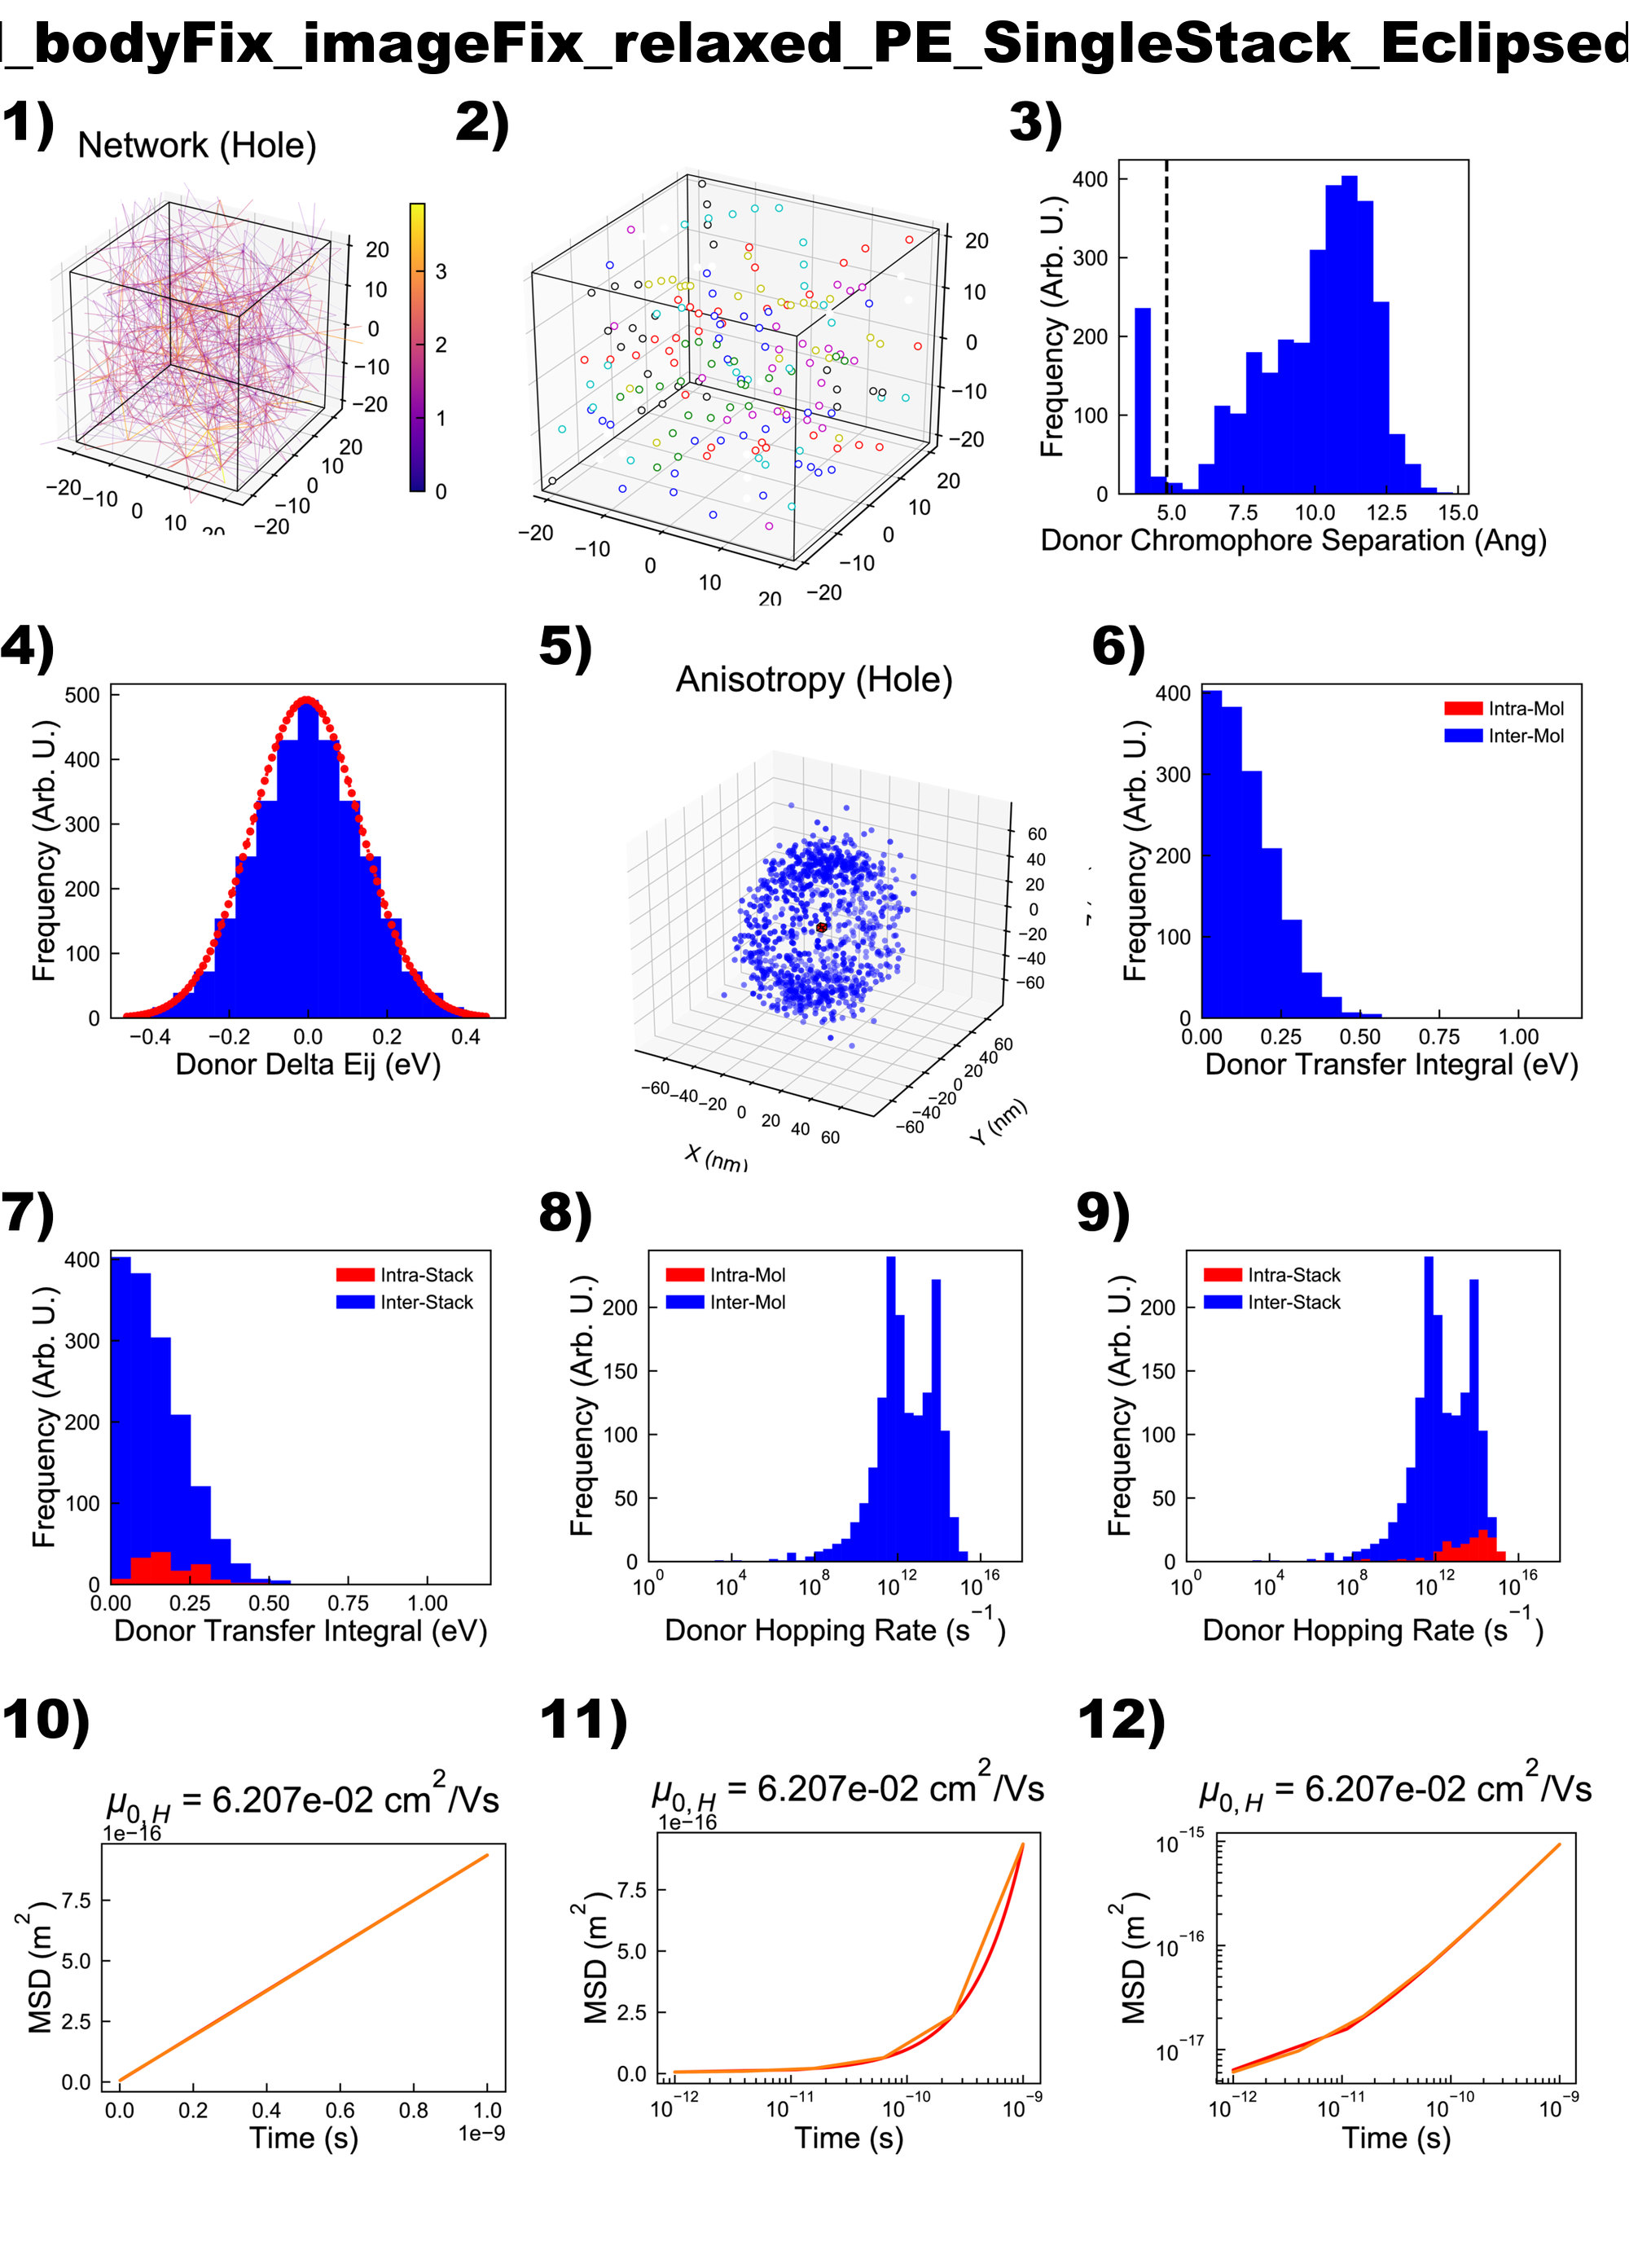
\includegraphics[width=0.85\textwidth]{Figures/VRH_bodyFix_imageFix_relaxed_PE_SingleStack_Eclipsed_AA.png}
    \caption{   1) Chromophore connectivity network, 
                2) Location of `stacks', 
                3) Distribution of connected chromophore separations (defines stacks),
                4) Density of states of Frontier molecular orbital (delta Eij),
                5) KMC Carrier termination locations (defines anisotropy),
                6) Histogram of molecular transfer integrals,
                7) Histogram of stack transfer integrals,
                8) Histogram of molecular hopping rates,
                9) Histogram of stack hopping rates,
                10) Linear MSD plot,
                11) Semi-log-x MSD plot,
                12) Logarithmic MSD plot.}
	\label{fig:VRHPESingEcl}
\end{figure}


\begin{figure}[h]\centering
	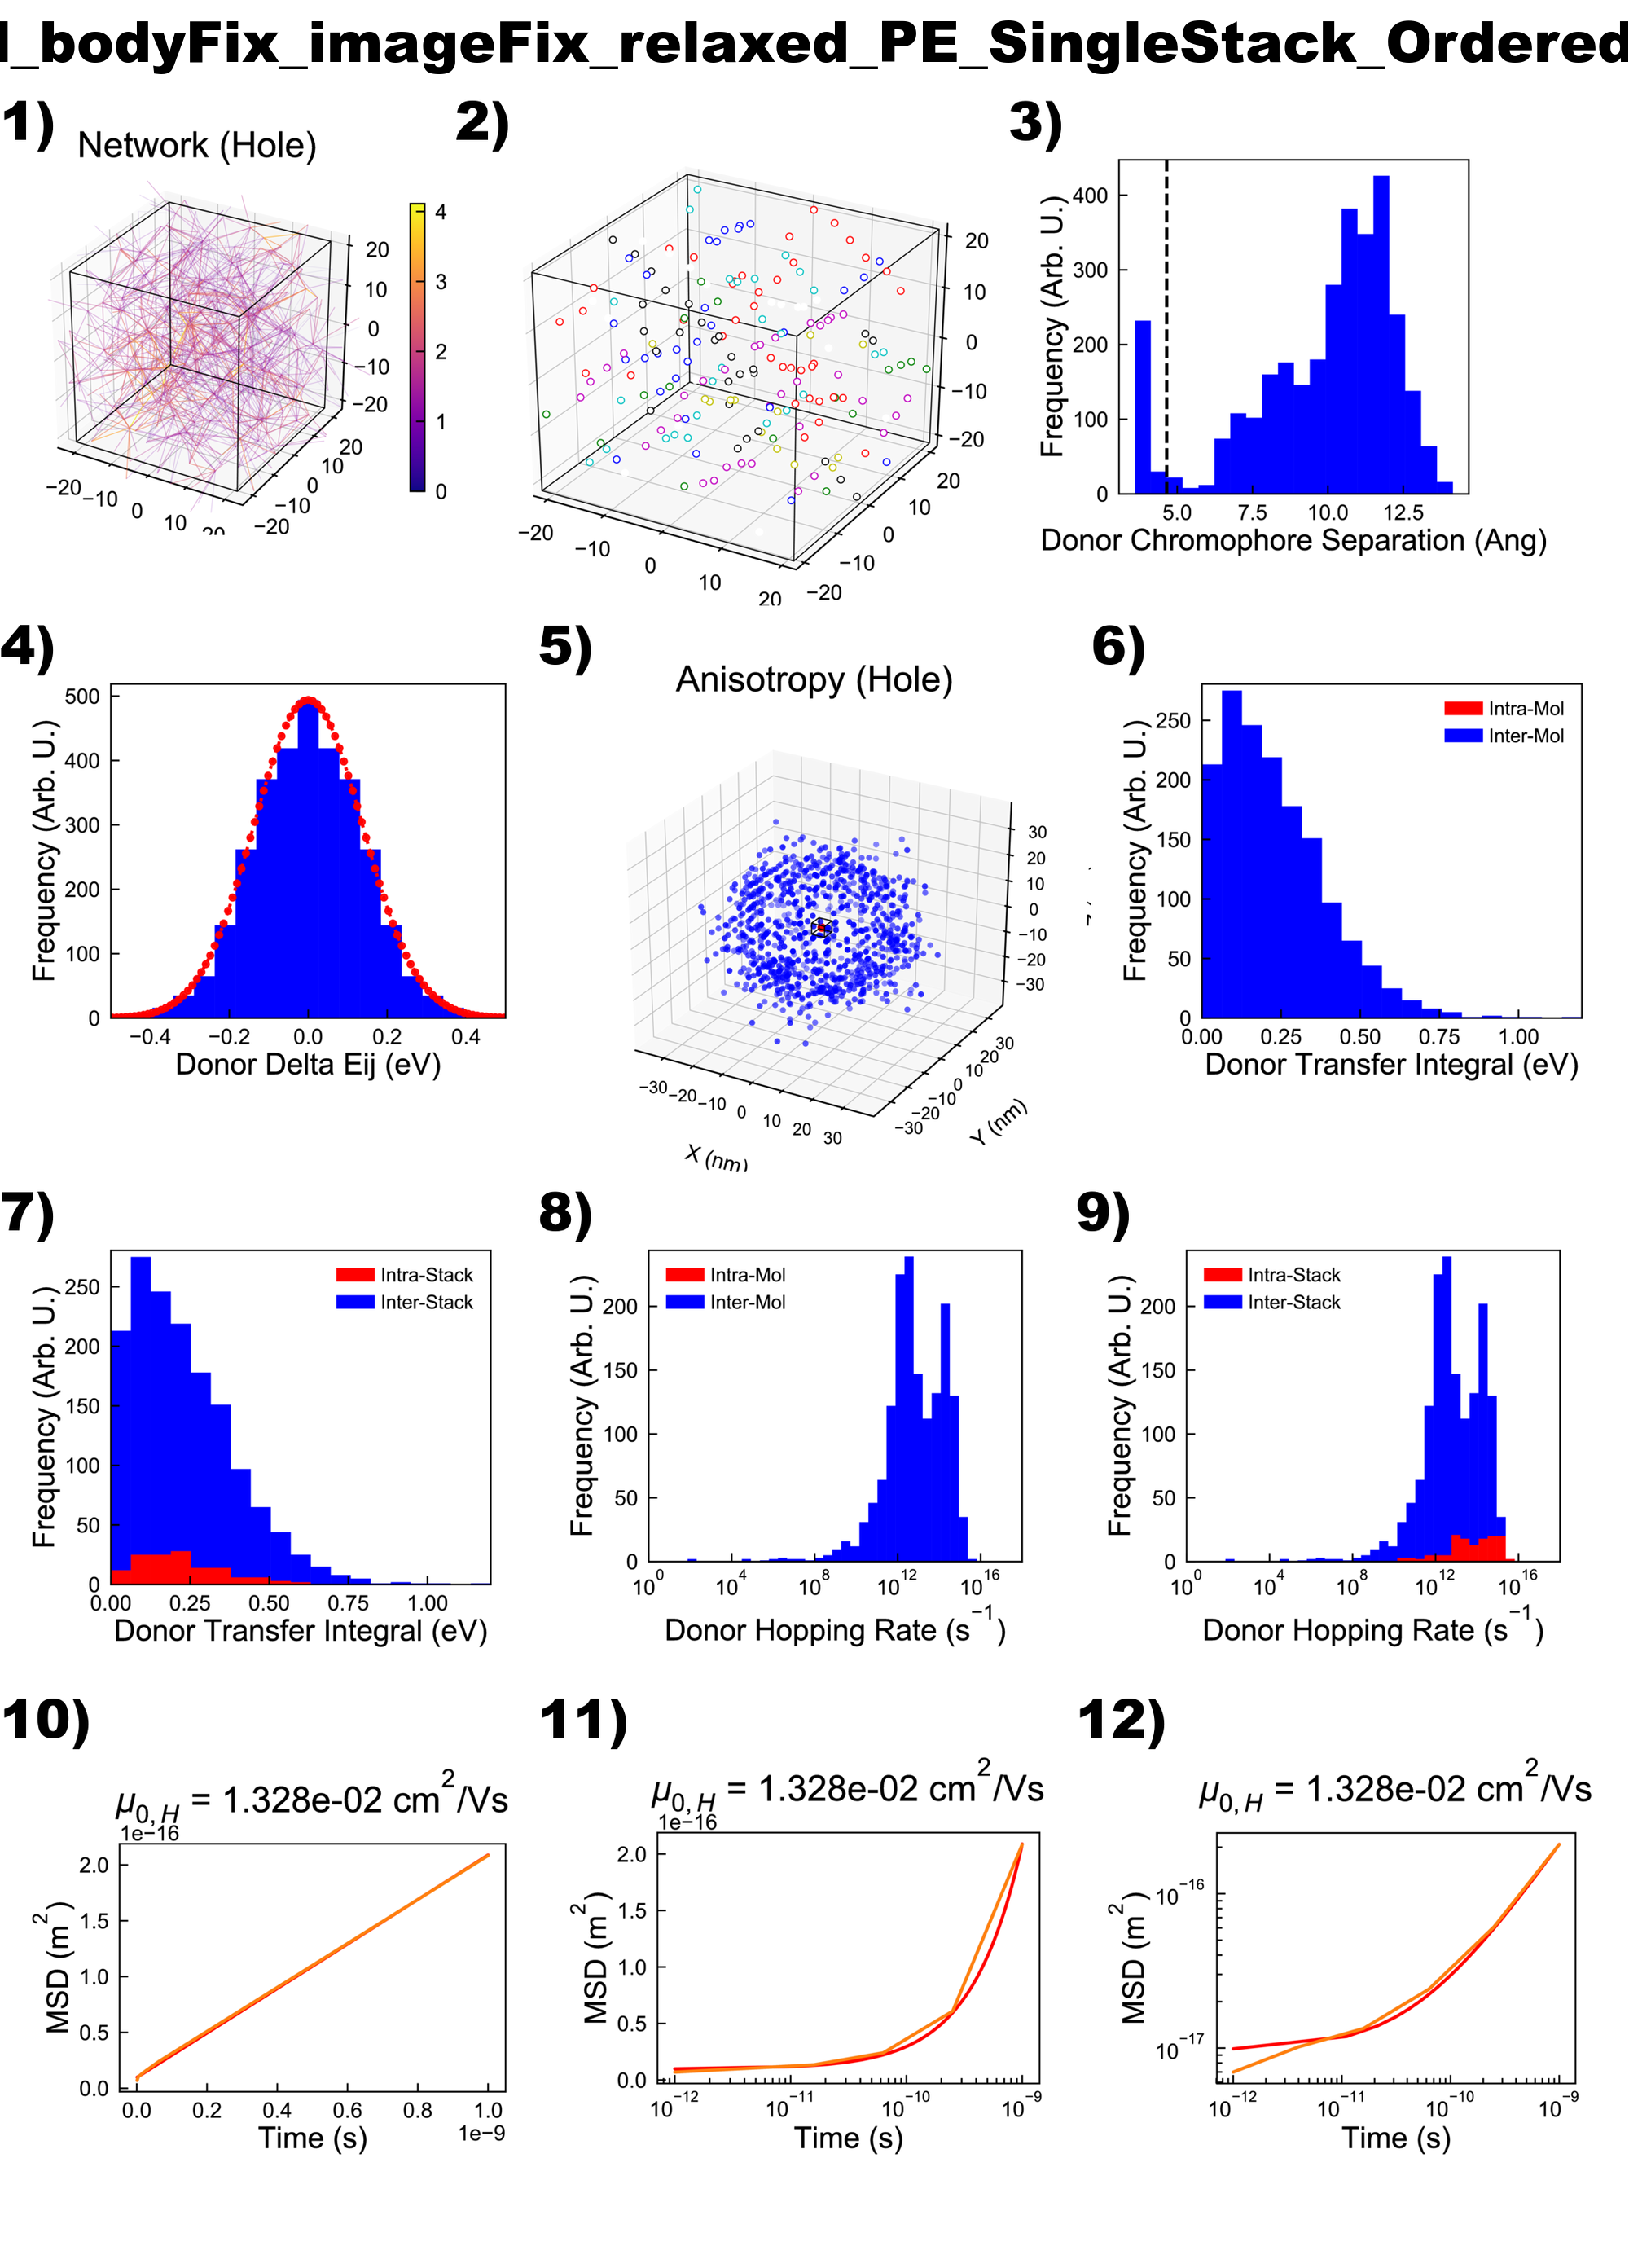
\includegraphics[width=0.85\textwidth]{Figures/VRH_bodyFix_imageFix_relaxed_PE_SingleStack_Ordered_AA.png}
    \caption{   1) Chromophore connectivity network, 
                2) Location of `stacks', 
                3) Distribution of connected chromophore separations (defines stacks),
                4) Density of states of Frontier molecular orbital (delta Eij),
                5) KMC Carrier termination locations (defines anisotropy),
                6) Histogram of molecular transfer integrals,
                7) Histogram of stack transfer integrals,
                8) Histogram of molecular hopping rates,
                9) Histogram of stack hopping rates,
                10) Linear MSD plot,
                11) Semi-log-x MSD plot,
                12) Logarithmic MSD plot.}
	\label{fig:VRHPESingOrd}
\end{figure}


\begin{figure}[h]\centering
	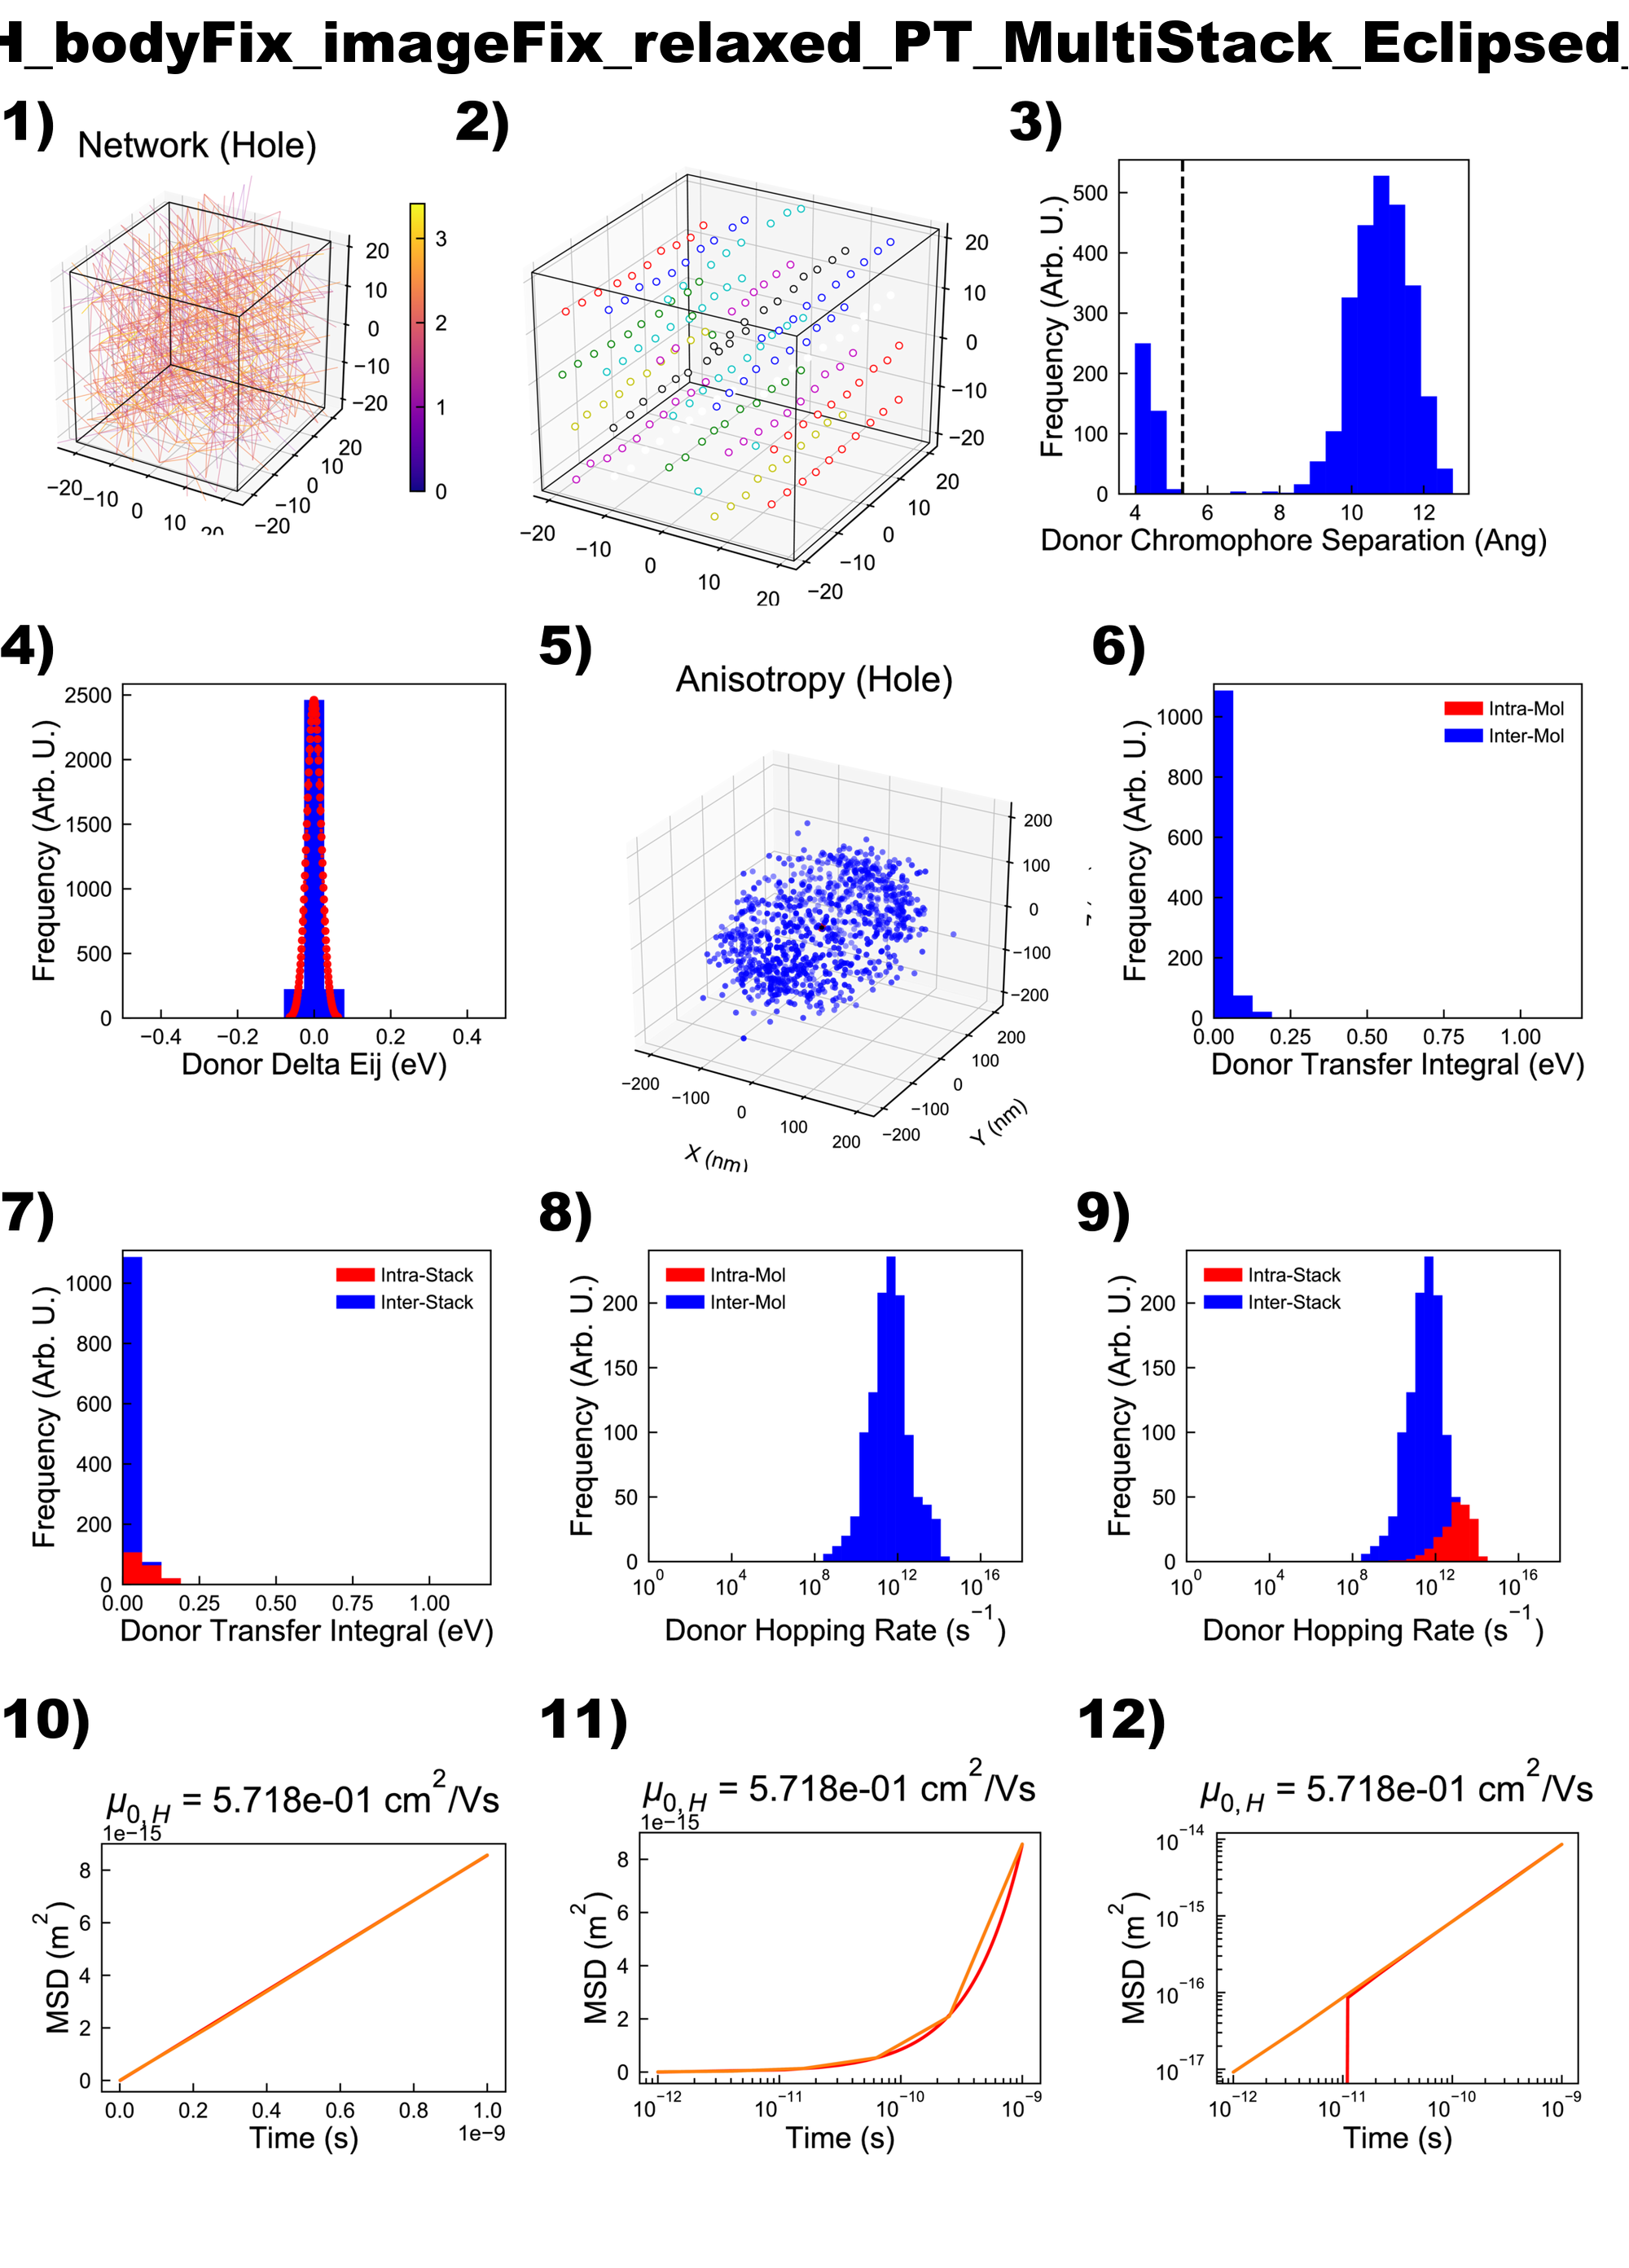
\includegraphics[width=0.85\textwidth]{Figures/VRH_bodyFix_imageFix_relaxed_PT_MultiStack_Eclipsed_AA.png}
    \caption{   1) Chromophore connectivity network, 
                2) Location of `stacks', 
                3) Distribution of connected chromophore separations (defines stacks),
                4) Density of states of Frontier molecular orbital (delta Eij),
                5) KMC Carrier termination locations (defines anisotropy),
                6) Histogram of molecular transfer integrals,
                7) Histogram of stack transfer integrals,
                8) Histogram of molecular hopping rates,
                9) Histogram of stack hopping rates,
                10) Linear MSD plot,
                11) Semi-log-x MSD plot,
                12) Logarithmic MSD plot.}
	\label{fig:VRHPTMultEcl}
\end{figure}


\begin{figure}[h]\centering
	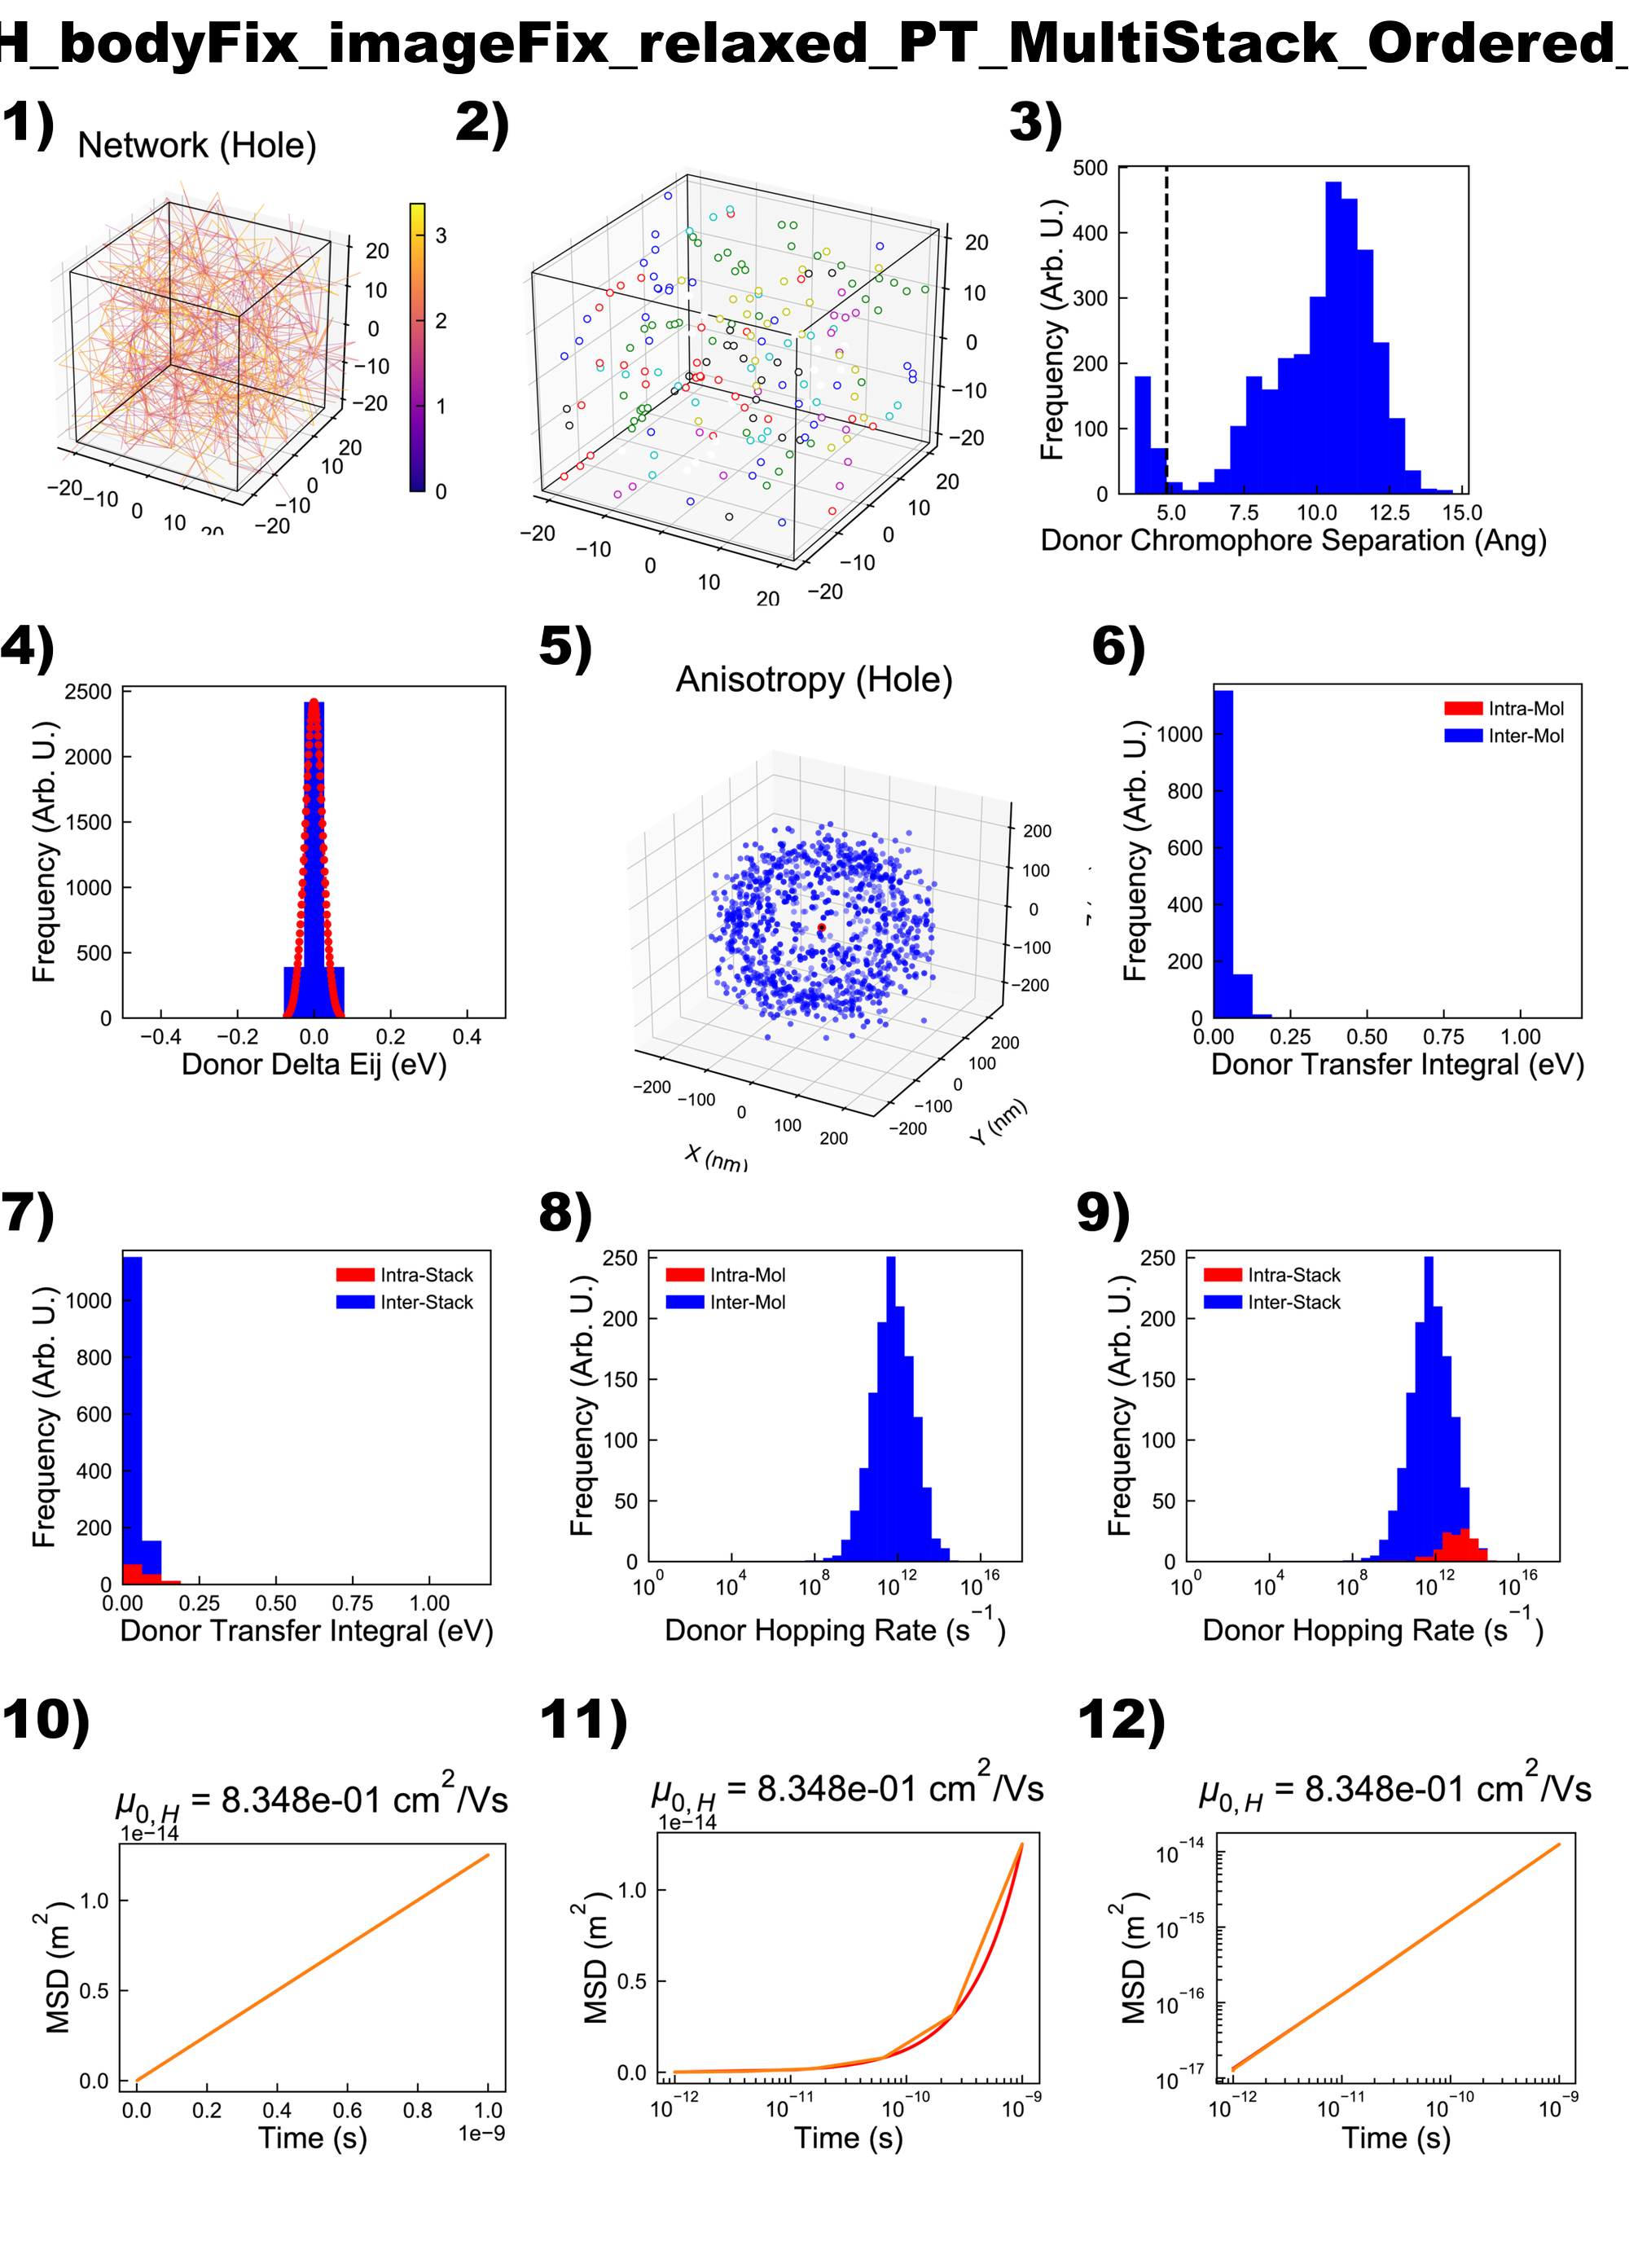
\includegraphics[width=0.85\textwidth]{Figures/VRH_bodyFix_imageFix_relaxed_PT_MultiStack_Ordered_AA.png}
    \caption{   1) Chromophore connectivity network, 
                2) Location of `stacks', 
                3) Distribution of connected chromophore separations (defines stacks),
                4) Density of states of Frontier molecular orbital (delta Eij),
                5) KMC Carrier termination locations (defines anisotropy),
                6) Histogram of molecular transfer integrals,
                7) Histogram of stack transfer integrals,
                8) Histogram of molecular hopping rates,
                9) Histogram of stack hopping rates,
                10) Linear MSD plot,
                11) Semi-log-x MSD plot,
                12) Logarithmic MSD plot.}
	\label{fig:VRHPTMultOrd}
\end{figure}


\begin{figure}[h]\centering
	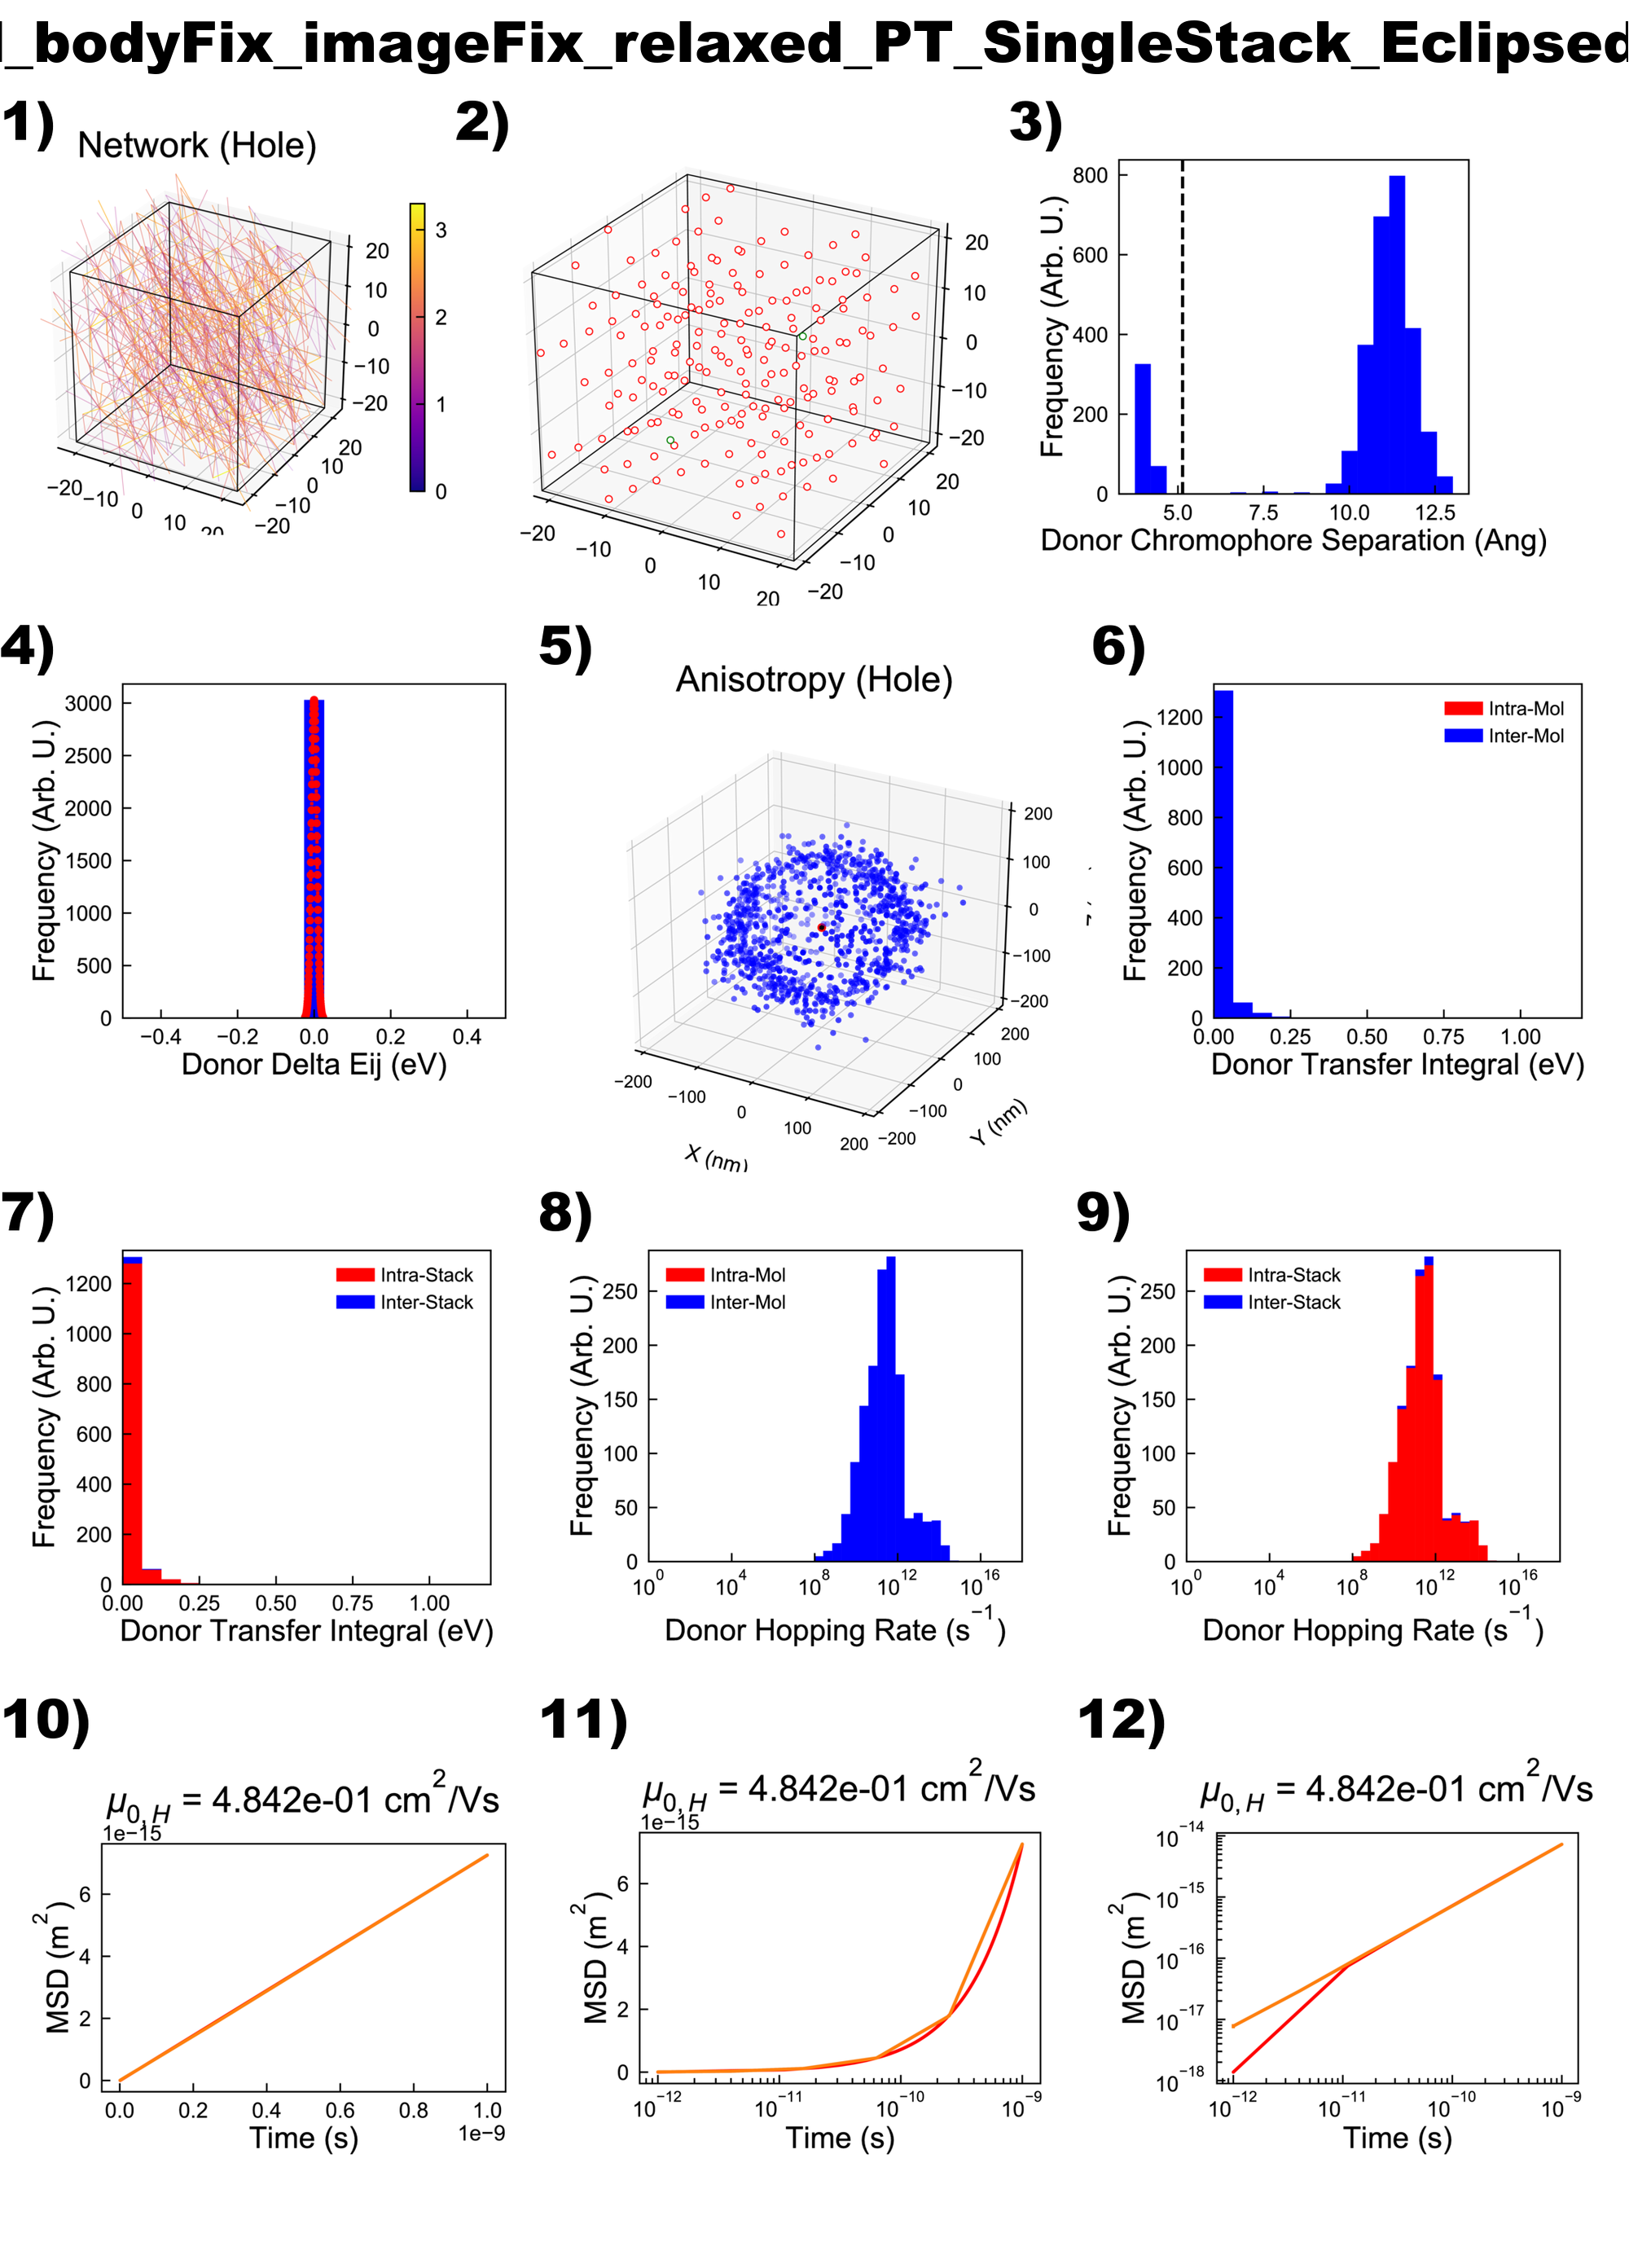
\includegraphics[width=0.85\textwidth]{Figures/VRH_bodyFix_imageFix_relaxed_PT_SingleStack_Eclipsed_AA.png}
    \caption{   1) Chromophore connectivity network, 
                2) Location of `stacks', 
                3) Distribution of connected chromophore separations (defines stacks),
                4) Density of states of Frontier molecular orbital (delta Eij),
                5) KMC Carrier termination locations (defines anisotropy),
                6) Histogram of molecular transfer integrals,
                7) Histogram of stack transfer integrals,
                8) Histogram of molecular hopping rates,
                9) Histogram of stack hopping rates,
                10) Linear MSD plot,
                11) Semi-log-x MSD plot,
                12) Logarithmic MSD plot.}
	\label{fig:VRHPTSingEcl}
\end{figure}


\begin{figure}[h]\centering
	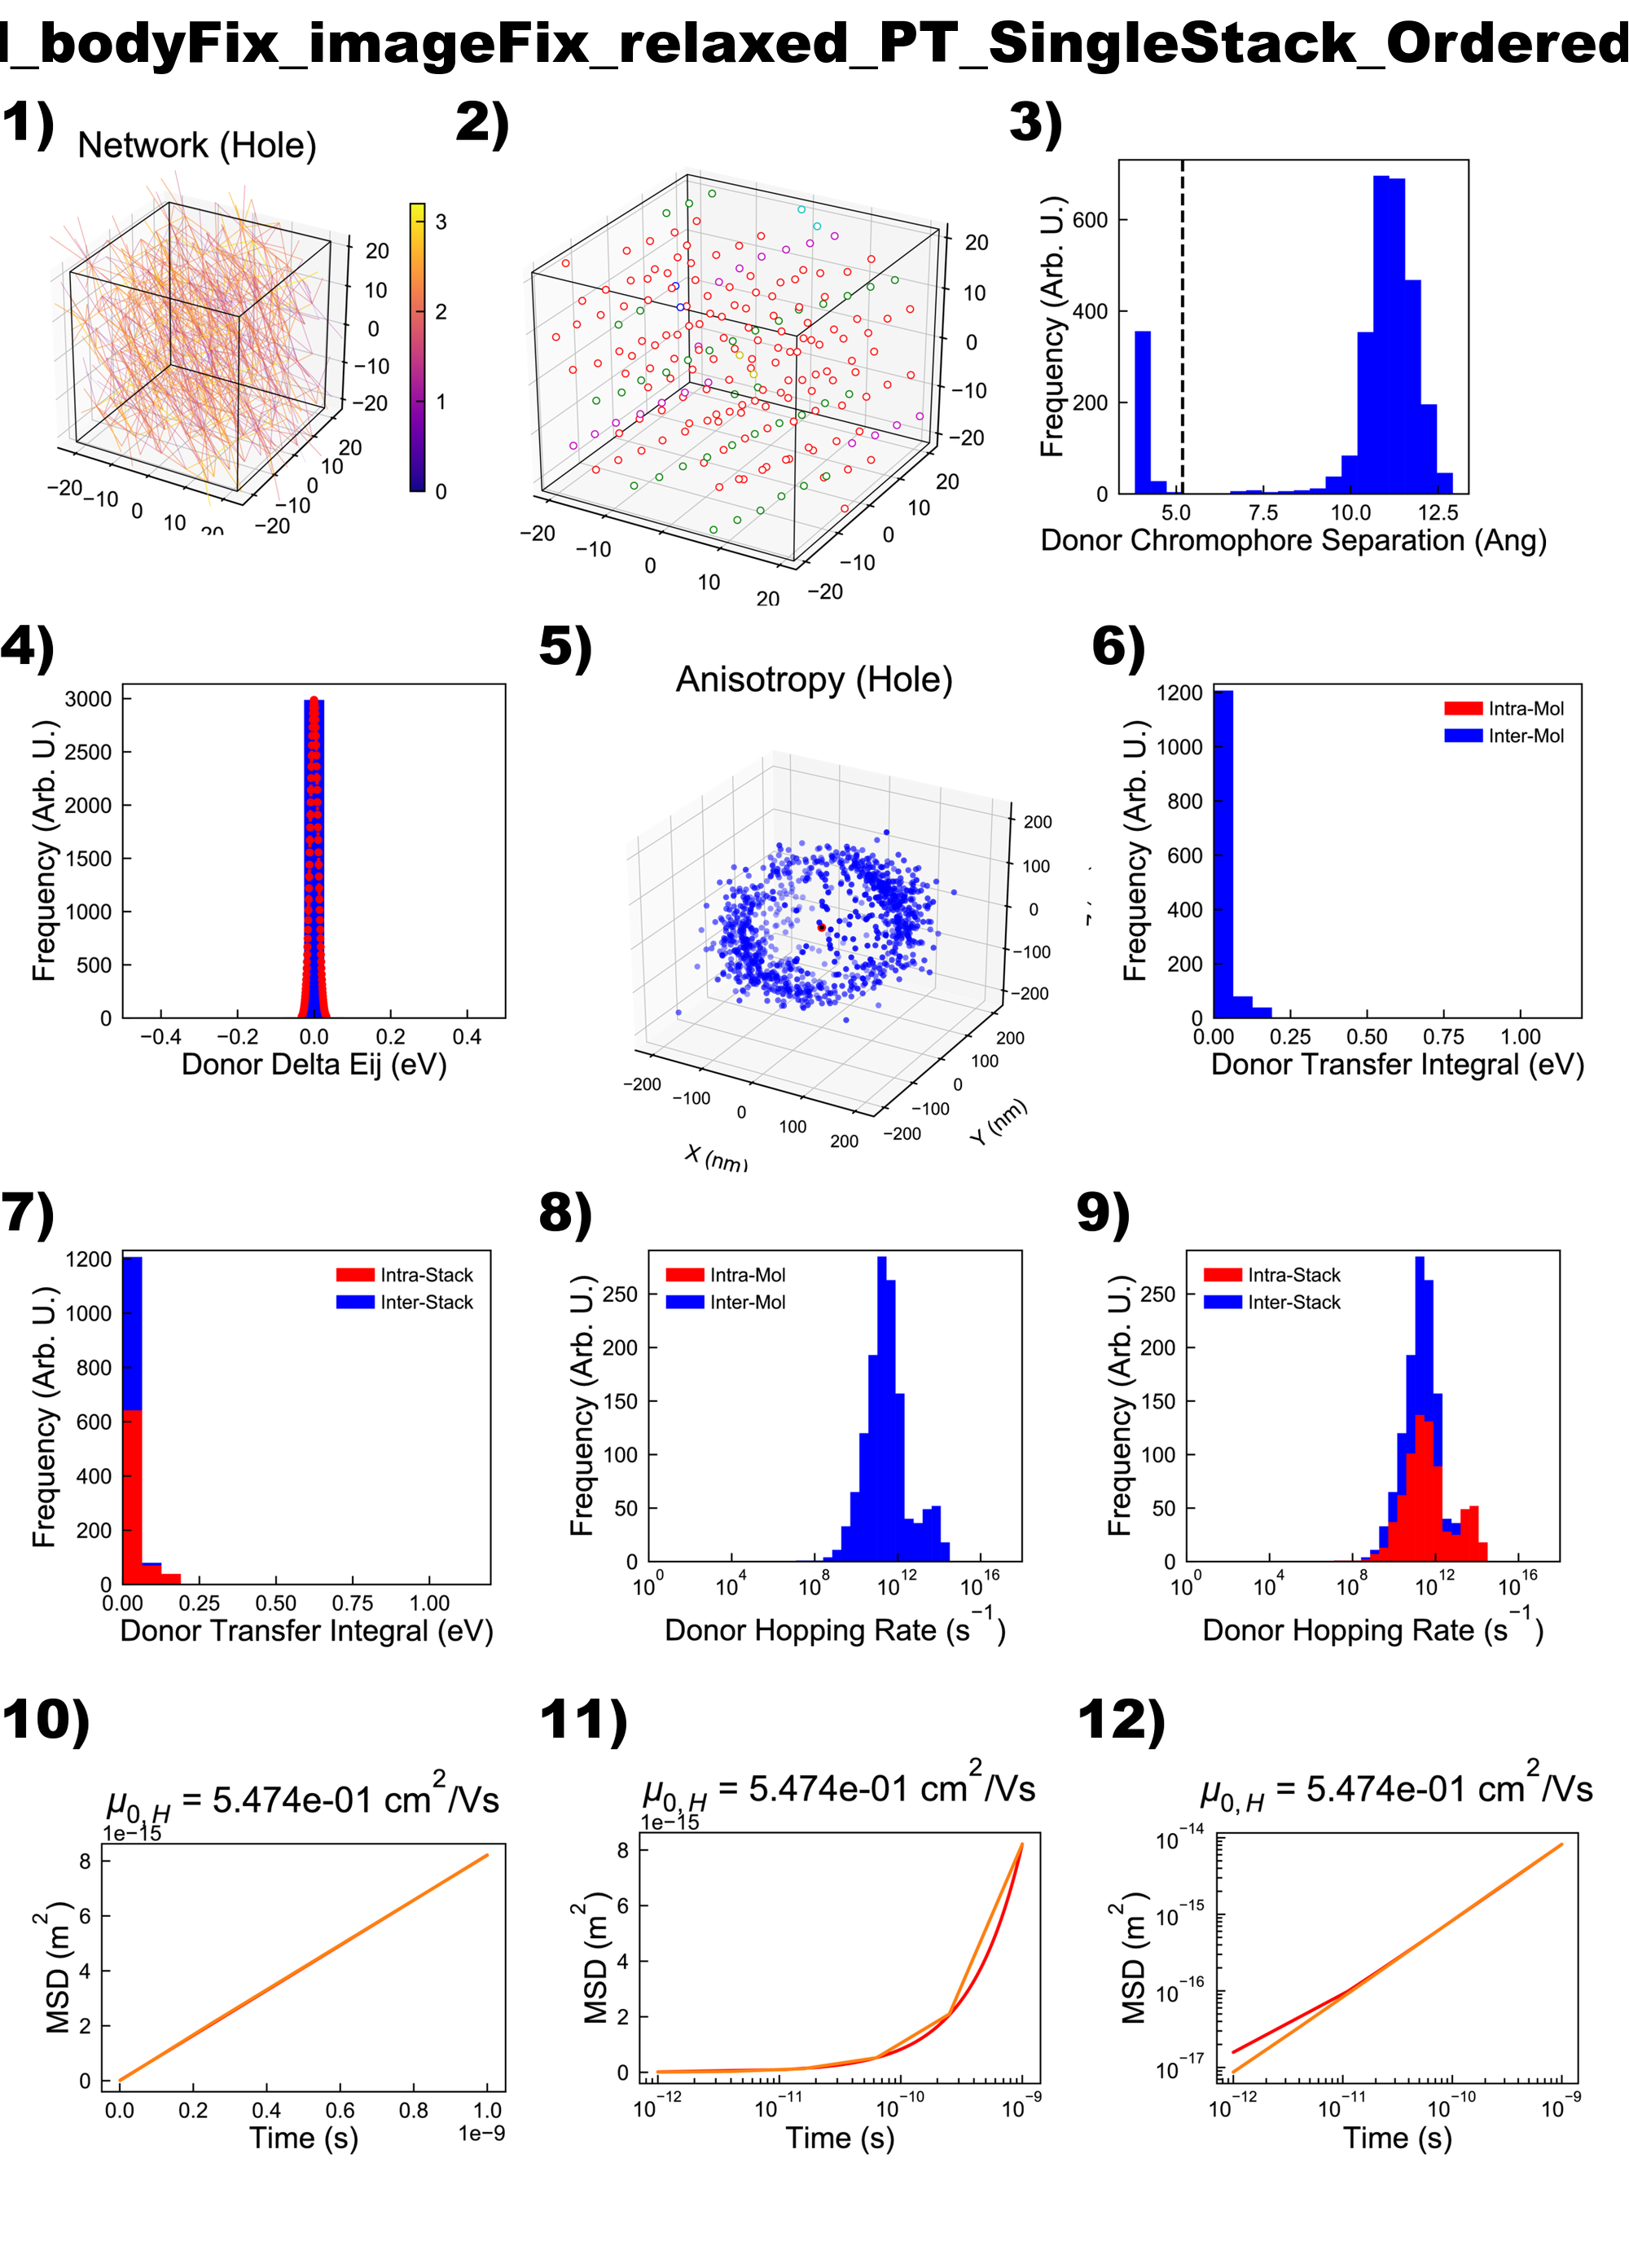
\includegraphics[width=0.85\textwidth]{Figures/VRH_bodyFix_imageFix_relaxed_PT_SingleStack_Ordered_AA.png}
    \caption{   1) Chromophore connectivity network, 
                2) Location of `stacks', 
                3) Distribution of connected chromophore separations (defines stacks),
                4) Density of states of Frontier molecular orbital (delta Eij),
                5) KMC Carrier termination locations (defines anisotropy),
                6) Histogram of molecular transfer integrals,
                7) Histogram of stack transfer integrals,
                8) Histogram of molecular hopping rates,
                9) Histogram of stack hopping rates,
                10) Linear MSD plot,
                11) Semi-log-x MSD plot,
                12) Logarithmic MSD plot.}
	\label{fig:VRHPTSingOrd}
\end{figure}

\bibliography{refs}
\bibliographystyle{unsrt}


\end{document}
